\documentclass{article}
\usepackage{amsmath}
\usepackage{mathrsfs}
\usepackage{amssymb}
\usepackage{bbm}
\usepackage{fancyhdr}
\usepackage{graphicx}
\usepackage{subcaption}
\usepackage{natbib}
\usepackage{booktabs}
\usepackage{url}
\usepackage{hyperref}
\graphicspath{ {./Billeder/} }

\hypersetup{
    colorlinks=true,
    linkcolor=blue,       % color for internal links (sections, equations)
    citecolor=blue,       % color for citations
    urlcolor=blue         % color for URLs
}

\begin{document}
\pagenumbering{roman}
\tableofcontents
\newpage
\pagenumbering{arabic}
\section{Introduction}
When modelling prices of financial assets, modelling the volatility process itself plays a crucial role. In the derivates world, log-prices are often modelled as continuous semi-martingales. For a given asset with log-price $Y_t$, such a process takes the form
\begin{align}
dY_t = \mu_tdt+\sigma_tdW_t
\end{align}
where $\mu_t$ is a drift term and $W_t$ is a one-dimensional Brownian motion. The term $\sigma_t$ represents the volatility process, and it is a very important ingredient in the model \cite{gatheral}. However, modelling the volatility process itself is also a complex task. Different approaches to estimate $\sigma_t$ is used in the literature. In the simplest models, the volatility is either constant or a deterministic function of time. In more popular stochastic volatility models, the volatility process is modelled as a stochastic process itself. In notable models such as the Hull and White model, the Heston model, and the SABR model, the volatility $\sigma_t$ is modelled as a continuous Brownian semi-martingale \cite{gatheral}. The stochastic volatility models seem way more realistic but generated prices from these models are in many cases not consistent with observed prices. (33, 46)\\\\
Various authors have proposed other kinds of models to model the volatility. A popular one is stochastic volatility models driven  by fractional Brownian motion. A well-known example of such a fractional stochastic volatility model is the one proposed by \cite{comte} who models the dynamics of the volatility $\sigma_t$ of an asset as:
\begin{align}
Y_t = \ln\sigma_t, \quad dY_t = -\gamma Y_t dt+\theta dB^H_t
\end{align}
where $B^H$ is a fractional Brownian motion with Hurst exponent $H$. The model was first introduced in order to model long range dependence effect observed in financial time series. The long range dependence is modelled by choosing $1>H>\frac{1}{2}$ \cite{comte}. In recent literature starting with \cite{gatheral}, it has been suggested to use the fractional stochastic volatility models with $H<\frac{1}{2}$ for modelling volatility. Processes driven by a fractional Brownian motion with $H<\frac{1}{2}$ are referred to as 'rough processes' since these fractional Brownian motion have trajectories rougher than a standard Brownian motion \cite{cont}, and \cite{gatheral} concludes that volatility is rough. It is important to note that \cite{gatheral} unlike previous literature rely on the behaviour of volatility estimators over short intraday time scales in order to asses the 'roughness'.\\\\
\cite{cont} challenges the conclusions of \cite{gatheral} and similar articles concluding that volatility is rough. \cite{cont} simulates from models where the true spot volatility is known and shows that measures of roughness for realized volatility based on the data from these simulations are in many cases much rougher than those of the underlying true spot volatility. This difference solely lies in the estimation error, and challenges the use of high-frequency volatility estimators when measuring the roughness.\\\\
In this thesis, we will take a similar approach as in \cite{cont} and investigate further if volatility appears to be rough even when the true model does not exhibit rough behaviour. 
\section{Fractional Brownian motion}
A fractional Brownian motion (fBm) $(B_t^H)_{t\in\mathbb{R}}$ with Hurst parameter $H\in(0,1)$ is a centered continuous Gaussian process with covariance function
\begin{align}
\mathbb{E}\left[B_t^HB_s^H\right] = \frac{1}{2}\left(t^{2H}+S^{2H}-\vert t-s\vert ^{2H} \right)
\end{align}
for $s,t\geq 0$. Note that $B_t^H$ reduces to an ordinary Brownian motion for $H = \frac{1}{2}$ \cite{dieker}. The incremental process of a fractional Brownian motion is called fractional Gaussian noise, and it is a stationary discrete-time process. We define the fractional Gaussian noise $X=\{X_k: k=0,1,...\}$ by 
\begin{align}
X_k:= B^H_{t_{k+1}}-B^H_{t_k}.
\end{align}
With this definition, we immediately see that every $X_k$ is normally distribution with mean 0 and variance 
\begin{align*}
&\mathbb{E}\left[ (B^H_{t_{k+1}}-B^H_{t_k})^2 \right] = Var (B^H_{t_{k+1}}) + Var(B^H_{t_k}) - 2Cov(B^H_{t_{k+1}}, B^H_{t_k})\\
&= t_{k+1}^{2H}+t_k^{2H} - \left( t_{k+1}^{2H}+t_k^{2H} - (t_{k+1}-t_k)^{2H} \right) = (t_{k+1}-t_k)^{2H}
\end{align*}
 using the covariance function (3). Thus, the fractional Gaussian noise is standard normal distributed when the time step is 1. 
\subsection{Simulation of fractional Brownian motion}
Throughout this thesis we will be simulating from the fractional Brownian motion by using a spectral method which can be used for stationary processes. The idea is to analyse the stochastic process in the spectral domain rather than the time domain. The spectral density is computed as follows for frequencies $-\pi\leq \lambda \leq \pi$:
\begin{align}
f(\lambda):= \sum_{j=-\infty}^\infty \gamma(j) \exp(ij\lambda)
\end{align}
where $\gamma(\cdot)$ represent the autocovariance function. It can be shown that the spectral density of fractional Gaussian noise is given by
\begin{align}
f(\lambda) = 2\sin(\pi H)\Gamma(2H+1)(1-\cos\lambda)[\vert\lambda\vert ^{-2H-1}+B(\lambda, H)]
\end{align}
where $\Gamma(\cdot)$ denotes the Gamma function and 
\begin{align}
B(\lambda, H) := \sum_{j=1}^\infty \left((2\pi j+\lambda)^{-2H-1}+(2\pi j-\lambda)^{-2H-1}\right)
\end{align}
for $-\pi\leq \lambda \leq \pi$. The infinite sum makes direct numerical evaluation almost impossible. However, a useful approximation of the sum is made by \cite{paxson}. They show that by using
\begin{align*}
&\tilde{B}_3(\lambda, H) :=\\ 
&\sum_{j=1}^3 \left(\left(a_j^+\right)^{-2H-1}+\left(a_j^-\right)^{-2H-1}\right)+\frac{\left(a_3^+\right)^{-2H}+\left(a_3^-\right)^{-2H}+\left(a_4^+\right)^{-2H}+\left(a_4^-\right)^{-2H}}{8H\pi}
\end{align*}
where $a^{\pm}_j=2\pi j\pm \lambda$, $f(\lambda)$ is approximated quite well.\\\\
Now, consider a stationary Gaussian discrete-time process $X=\{X_n: n = 0,...,N-1\}$ where $N$ is the required sample size. The spectral theorem states that it can be represented in terms of the spectral density as
\begin{align}
X_n\overset{d}{=}\int_0^\pi \sqrt{\frac{f(\lambda)}{\pi}}\cos(n\lambda)dB_1(\lambda)-\int_0^\pi \sqrt{\frac{f(\lambda)}{\pi}}\sin(n\lambda)dB_2(\lambda)
\end{align}
where $B_1$ and $B_2$ are two mutually independent Brownian motions \cite{dieker}. We wish to approximate (8). The integrand is replaced by a simpler function. Fix some integer $l$ and set $t_k = \pi k/l$ for $k=0,...,l$. Now, define a simple function $\xi_n^{(l)}$ on $[0,\pi]$ for $0\leq n\leq N-1$ by 
\begin{align}
\xi_n^{(\ell)}(\lambda)= \sqrt{\frac{f(t_1)}{\pi}}\cos(nt_1)\mathbf{1}_{\{0\}}(\lambda)+\sum_{k=0}^{l-1} \sqrt{\frac{f(t_{k+1})}{\pi}}\cos(nt_{k+1})\mathbf{1}_{(t_k,t_{k+1}]}(\lambda).
\end{align}
The first integral in $(8)$ can be approximated by $\int_0^\pi \xi_n^{(\ell)}(\lambda)dB_1(\lambda)$. Since $\xi_n^{(\ell)}$ is a simple function the stochastic integral can be computed as
\begin{align}
\int_0^\pi \xi_n^{(l)}(\lambda)dB_1(\lambda) = \sum _{j=0}^{\ell-1} \xi_n^{(l)} (B(t_{j+1})-B(t_j)).
\end{align} 
Thus, we obtain 
\begin{align*}
&\int_0^\pi \xi_n^{(l)}(\lambda)dB_1(\lambda) = \sum_{j=0}^{\ell-1}\sum_{k=0}^{\ell-1} \sqrt{\frac{f(t_{k+1})}{\pi}} \cos(n t_{k+1}) \mathbf{1}_{(t_k,t_{k+1}]}(B_1(t_{j+1})-B_1(t_j))\\
&= \sum_{k=0}^{l-1} \sqrt{\frac{f(t_{k+1})}{\pi}} \cos(n t_{k+1}) 
(B_1(t_{k+1})-B_1(t_k)) \\
&= \sum_{k=0}^{\ell-1} \sqrt{\frac{f(t_{k+1})}{\pi}} \cos(n t_{k+1})U_k^{(0)} \sqrt{\frac{\pi}{l}} = \sum_{k=0}^{\ell-1} \sqrt{\frac{f(t_{k+1})}{\ell}} \cos(n t_{k+1})U_k^{(0)}
\end{align*}
where $U_k^{(0)}$ is an i.i.d. standard normal random variable for $k=0,...,\ell-1$. The $U_k^{(0)}\sqrt{\pi/\ell}$ represent the Brownian motion increments which per definition are normally distributed with mean $0$ and variance $t_{k+1}-t_k$.\\\\
The second integral in $(8)$ can be approximated in a similar way by replacing the cosine terms with sine terms. Thus, we obtain the following approximation of $X_n$:
\begin{align}
\hat{X}_n^{(\ell)} := \sum_{k=0}^{\ell-1} \sqrt{\frac{f(t_{k+1})}{\ell}}\left( \cos(nt_{k+1})U_k^{(0)}-\sin (nt_{k+1}) U_k^{(1)}\right).
\end{align}
The two vectors $U^{(0)}$ and $U^{(1)}$ are mutually independent since $B_1$ and $B_2$ are independent as well. In order to calculate $\hat{X}_n^{(\ell)}$ efficiently we will be using the fast Fourier transform (FFT). To this end, we define the sequence $(a_k)_{k=0,...,2\ell-1}$ by

\[
a_k := \begin{cases}
0 & k = 0; \\
\frac{1}{2} \left( U^{(0)}_{k-1} + i U^{(1)}_{k-1} \right) \sqrt{\frac{f(t_k)}{\ell}} & k = 1, \dots, \ell - 1; \\
U^{(0)}_{k-1} \sqrt{\frac{f(t_k)}{\ell}} & k = \ell; \\
\frac{1}{2} \left( U^{(0)}_{2\ell - k - 1} - i U^{(1)}_{2\ell - k - 1} \right) \sqrt{\frac{f(t_{2\ell - k})}{\ell}} & k = \ell + 1, \dots, 2\ell - 1.
\end{cases}
\]
It is shown in appendix that the Fourier transform of $a_k$ is indeed real and equals $\hat{X}_n^{(\ell)}$. From this approximated fractional Gaussian noise we can generate the fBm. \\

\cite{dieker} shows that the finite-dimensional distributions of $\hat{X}^{(\ell)}$ converge in probability to the corresponding finite-dimensional distributions of $X$ as $\ell\rightarrow \infty$. The rate of convergence is, however, quite slow. Therefore, we will be using a $\ell \geq 30000$ when simulating from the fBm by the spectral method in this thesis in order to make sure that our simulations are reliable. Figure \ref{fig:fbmsim} shows three simulations of fractional Brownian motions with different Hurst parameters generated by the spectral method. 
\begin{figure}[h]
    \centering
    \begin{subfigure}{0.32\textwidth}
        \centering
        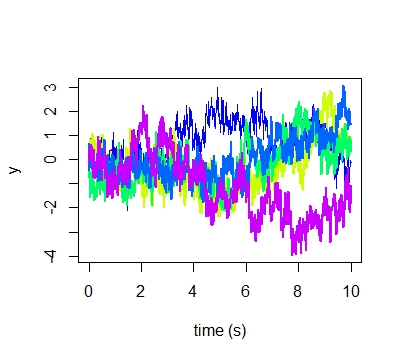
\includegraphics[width=\textwidth]{specsim1.jpeg}
        \caption{H=0.2}
    \end{subfigure}\hfill
    \begin{subfigure}{0.32\textwidth}
        \centering
        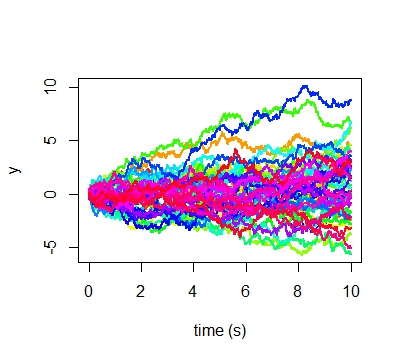
\includegraphics[width=\textwidth]{specsim2.jpeg}
        \caption{H=0.5}
    \end{subfigure}\hfill
    \begin{subfigure}{0.32\textwidth}
        \centering
        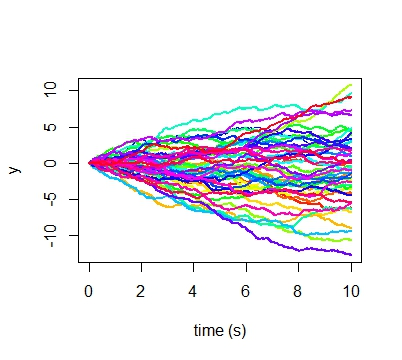
\includegraphics[width=\textwidth]{specsim3.jpeg}
        \caption{H=0.8}
    \end{subfigure}
    \caption{Fractional Brownian motions generated by the spectral method.}
    \label{fig:fbmsim}
\end{figure}

\section{Estimating the roughness of volatility}
Determining the roughness of volatility plays a crucial role in order to make proper model specification and design estimators. In practice when estimating the roughness, we observe only a singe price path, and we need to measure the roughness of this path. Estimating the roughness from discrete observation is not an easy task and multiple ways of estimating the roughness exist in the literature. In this thesis, we will be working with high frequency data, and we will introduce three different roughness estimators that works on high frequency data. In section 4 we will conduct numerical experiments, and we will compare the three estimators. 
\subsection{Roughness index estimator via $p$-th variation}
In this section, we will describe the roughness index estimator via normalized $p$-th variation which was introduced in \cite{cont}. We will closely follow the theory and methodology behind the estimator described in \cite{cont}.\\

We will be working with partitions of our time interval. Consider a sequence of partitions $\pi = (\pi^n) _{n\geq 1}$ of $[0,T]$ where
\[
\pi^n = \left( 0 = t_0^n < t_1^n < ... < t^n_{N(\pi^n)}=T \right)
\]
represents observation times at frequency $n$. Here $N(\pi^n)$ denotes the number of intervals in the partition $\pi^n$. For the time partitions we will be working with in this thesis we will assume that 
\begin{align}
\lvert \pi^n \rvert := \sup_{i=1, \dots, N(\pi^n)} \lvert t_i^n - t_{i-1}^n \rvert \xrightarrow{n \to \infty} 0.
\end{align}
That is, the size of the largest interval of $\pi^n$ will converge to 0 as $n\rightarrow \infty$.

We will now define the concept of $p$-th variation along a sequence of partitions $(\pi^n) _{n\geq 1}$. The definition follows the definition from \cite{cont2}.\\\\ 
\textbf{Definition 1.} \textit{(p-th variation along a sequence of partitions) 
$x \in C^0([0,T], \mathbb{R})$ has finite p-th variation along the sequence of partitions 
$\pi = (\pi^n, n \geq 1)$ if there exists a continuous increasing function $[x]_{\pi}^{(p)}: [0,T] \to \mathbb{R}_+$ such that
\[
\forall t \in [0,T], \quad \sum_{\{t_j^n, t_{j+1}^n\} \in \pi^n: t_j^n \leq t} \lvert x(t_{j+1}^n) - x(t_j^n) \rvert^p 
\xrightarrow{n \to \infty} [x]_{\pi}^{(p)}(t). \tag{3}
\]
If this property holds, then the convergence in (3) is uniform. We call $[x]_{\pi}^{(p)}$ the p-th variation of $x$ along the sequence of partitions $\pi$. We denote $V_\pi^p([0,T], \mathbb{R})$ the set of all continuous paths with finite p-th variation along $\pi$.}\\\\
We further define the concepts of variation index and roughness index of a path following \cite{cont}. \\\\
\textbf{Definition 2} (Variation index). \textit{The variation index of a path $x$ along a partition sequence $\pi$ is defined as the smallest $p \geq 1$ for which $x$ has finite p-th variation along $\pi$:}
\[
p^{\pi}(x) = \inf \left\{ p \geq 1 : x \in V_{\pi}^p([0,T], \mathbb{R}) \right\}.
\]\\
\textbf{Definition 3} (Roughness index). \textit{The roughness index of a path $x$ (along $\pi$) is defined as}
\[
H^{\pi}(x) = \frac{1}{p^{\pi}(x)}.
\]\\
When the underlying sequence of partitions is clear, we will simply denote these indexes as $p(x)$ and $H(x)$. \\\\
For a real-valued stochastic process $X: [0,T]\times \Omega \rightarrow \mathbb{R}$ the variation index (hence also the roughness index) $p^\pi (X(.,\omega))$ of each sample path $X(.,\omega)$ may in principle be different. However, there are many important classes of stochastic processes which have an almost-sure roughness index. This holds for example for a fractional Brownian motion where the roughness index matches with the corresponding Hurst parameter \cite{cont}.\\\\
When estimating roughness from empirical data based on discrete observations, using the $p$-th variation directly is difficult since it involves checking convergence to an unknown limit. To this end, we introduce the concept of normalized $p$-th variation.\\\\
\textbf{Definition 4} (Normalized p-th variation along a sequence of partitions). 
\textit{Let $\pi$ be a sequence of partitions of $[0, T]$ with mesh $\lvert \pi^n \rvert \to 0$ and 
$\pi^n = \{ 0 = t_1^n < t_2^n < \cdots < t_{N(\pi^n)}^n = T \}$. 
$x \in V_{\pi}^p([0, T], \mathbb{R})$ is said to have normalized p-th variation along $\pi$ 
if there exists a continuous function $w(x, p, \pi) : [0, T] \to \mathbb{R}$ such that:}
\[
\forall t \in [0, T], \quad \sum_{\pi^n \cap [0,t]} \lvert x(t_{j+1}^n) - x(t_j^n) \rvert^p \to w(x, p, \pi)(t).
\]
(Cont and Das 2022) shows that for a large class of functions with $p$-th variation, the normalized $p$-th variation exists and is linear. Furthermore, \cite{cont} shows that the normalized $p$th variation is a 'sharp' statistic meaning that if a function has finite $p$-th variation then for all $q\neq p$ the normalized $p$-th variation is either zero or infinite. Additionally, it is shown that a fractional Brownian motion has normalized $p$-th variation along the dyadic partition $\mathbb{T}= (\mathbb{T}^n)_{n\geq 1}$ almost-surely.
\subsubsection{Estimating the roughness from discrete observations}
With these concepts defined we now proceed to explaining how roughness can be estimated from discrete observations. Given discrete observations on a refining partition $\pi^L$ we define the 'normalized $p$-th variation statistic' which is the discrete counterpart of the normalized $p$-th variation:
\begin{align}
W(L, K, \pi, p, t, X) := \sum_{\pi^K\cap [0,t] } \frac{\lvert X(t_{i+1}^K)-X(t_i^K)\rvert^p}{\sum_{\pi^L\cap [t_i^K, t_{i+1}^K]}\lvert X(t_{j+1}^L)-X(t_j^L)\rvert^p} \times (t_{i+1}^K-t_i^K).
\end{align}
This definition involves two frequencies $K$ and $L>>K$. We can consider $L$ as the sample frequency while $K$ is a block frequency such that $\pi^K$ is a subpartition of $\pi^L$. Thus, we are grouping the sample size $L$ into $K$ many groups where each group contains exactly $\frac{L}{K}$ consecutive points. It can be seen that the normalized $p$-th variation statistic converges to the normalized $p$-th variation as $L$ and $K$ increase. That is,
\begin{align}
\lim_{K\rightarrow\infty}\lim_{L\rightarrow\infty} W(L, K, \pi, p, t, X) = w(x, p, \pi)(t).
\end{align}
The variation index estimator $\hat{p}^\pi_{L,K}(X)$ associated with data sampled on $\pi^L$ can then be obtained by computing $W(L, K, \pi, p, t, X)$ for different values of $p$ such that the following equation can be solved for $p^\pi_{L,K}(X)$
\begin{align}
W(L, K, \pi, \hat{p}^\pi_{L,K}(X), t, X) = T. \label{eq:wpth}
\end{align}
The corresponding roughness index estimator is then defined as
\begin{align*}
\hat{H}^\pi_{L,K}(X) = \frac{1}{\hat{p}^\pi_{L,K}(X)}.
\end{align*}
If the underlying dataset and partition is clear we will also denote these estimators as $\hat{p}_{L,K}$ and $\hat{H}_{L,K}$. Asymptotic properties of these estimators under high-frequency sampling are studied in (cont and das 2022). 
\subsubsection{Behaviour of the roughness estimator based on simulations}
We will now study the behaviour of the roughness estimator based on high-frequency simulated data. We will be simulating from a fractional Brownian motion and compute the roughness estimator based on the data. In this simulation section we will be using a uniform partition of the time interval $[0,1]$ with
\begin{align*}
\pi^n = \left( 0 < \frac{1}{n}< \frac{2}{n}<...< 1\right).
\end{align*}
We will be simulating from four fractional Brownian motions with four different Hurst exponents $H=\{0.1,0.3,0.5,0.8\}$ in order to investigate the accuracy of the roughness estimator $\hat{H}^\pi_{L,K}(X)$. First, we plot $\log(W(L=300\times 300, K=300, \pi, p, t=1, X=B^H))$ against $H=1/p$ to visualize the estimation. The results are presented in Figure \ref{fig:checkw}. The solid black line is the value of $\log(W(L=300\times 300, K=300, \pi, p, t=1, X=B^H))$ for different values of $1/p$. The blue vertical line represents the estimated roughness index whereas the black dotted vertical line represent the true Hurst parameter. The blue horizontal line represents $W(L, K, \pi, p, t, X) = T$. The estimated roughness index $\hat{H}_{L,K}$ is the crossing between $\log(W(L=300\times 300, K=300, \pi, p, t=1, X=B^H))$ and $W(L, K, \pi, p, t, X) = T$. \\\\
\begin{figure}[htbp]
    \centering
    
    \begin{subfigure}{0.48\textwidth}
        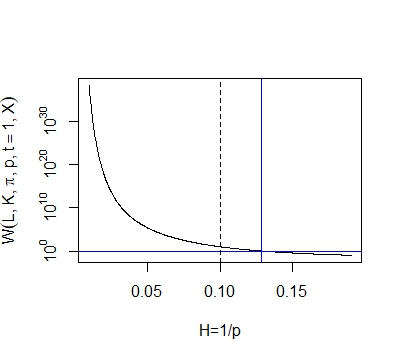
\includegraphics[width=\linewidth]{wagainstp_H01.jpeg}
    \end{subfigure}
    \hfill
    \begin{subfigure}{0.48\textwidth}
        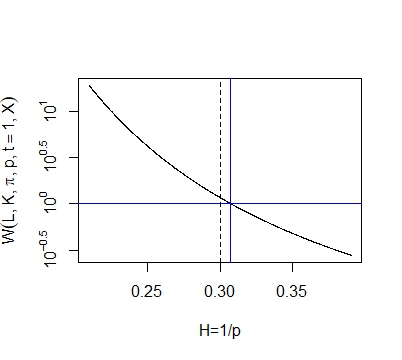
\includegraphics[width=\linewidth]{wagainstp_H03.jpeg}
    \end{subfigure}
    \vskip 0em
    \begin{subfigure}{0.48\textwidth}
        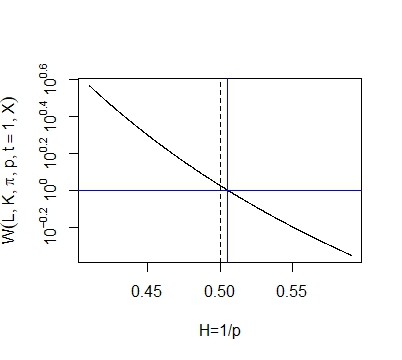
\includegraphics[width=\linewidth]{wagainstp_H05.jpeg}
    \end{subfigure}
    \hfill
    \begin{subfigure}{0.48\textwidth}
        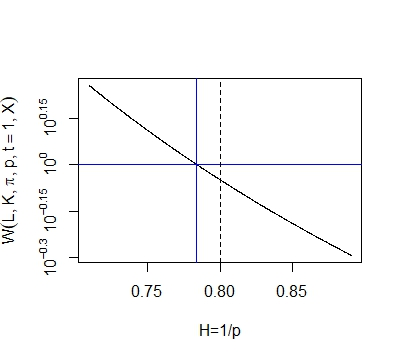
\includegraphics[width=\linewidth]{wagainstp_H08.jpeg}
    \end{subfigure}
    
    \caption{Log-scale plot of the normalized $p$-th variation statistic for fBm with Hurst parameter $H=\{0.1,0.3,0.5,0.8\}$. The black solid line represents the value of $\log(W(L=300\times 300, K=300, \pi, p, t=1, X=B^H))$ plotted against $H=1/p$. The blue vertical line represents $\hat{H}_{L,K}$ using the normalized $p$-th variation statistic with $L=300\times 300$ and $K=300$. The vertical black dotted line represents the true Hurst parameter. }
    \label{fig:checkw}
\end{figure}
In Figure \ref{fig:checkhist}, we have created histograms of the estimator $\hat{H}_{L,K}$ again by using $W(L=300\times 300, K=300, \pi, p, t=1, X=B^H)$ from 150 independent simulations. In addition to this, Table \ref{tab:checkhist} provides the summary statistics for the estimated roughness index $\hat{H}_{L,K}$ shown in the histograms. Based on Figure \ref{fig:checkw} and \ref{fig:checkhist}, and Table \ref{tab:checkhist}, we conclude that the estimated roughness index $\hat{H}_{L,K}$ seems to be fairly accurate when used on a data set with length $L=300\times 300$ generated from a fractional Brownian motion. All the estimated  $\hat{H}_{L,K}$ are within a distance $0.05$ from the true Hurst parameter, and the mean and median of the estimated roughness are in all cases very close to the true Hurst parameter indicating that our estimator is quite accurate. Only exception is for the fBm with Hurst parameter $H=0.8$ where even the upper quartile of $\hat{H}_{L,K}$ is smaller than the true Hurst parameter as seen in Table \ref{tab:checkhist}. This suggest that the estimated roughness index might be biased downwards in the case of $H=0.8$. The estimate is, however, still quite accurate even for $H=0.8$.
\begin{table}[htbp]
    \centering
    \begin{tabular}{ccccccc}
        \toprule
        H & Min. & Lower quartile & Median & Mean & Upper quartile & Max. \\
        \midrule
        0.1 & 0.0622 & 0.0944 & 0.1021 & 0.1031 & 0.1149 & 0.1402 \\
        0.3 & 0.2746 & 0.2954 & 0.3012 & 0.3005 & 0.3052 & 0.3177 \\
        0.5 & 0.4743 & 0.4954 & 0.5004 & 0.4997 & 0.5041 & 0.5239 \\
        0.8 & 0.7657 & 0.7797 & 0.7856 & 0.7865 & 0.7937 & 0.8239 \\
        \bottomrule
    \end{tabular}
    \caption{Summary of statistics for estimated roughness index $\hat{H}_{L,K}$ from 150 independent simulations of fBm with $L=300\times 300$ and $K=300$.}
    \label{tab:checkhist}
\end{table}
\begin{figure}[htbp]
    \centering
    
    \begin{subfigure}{0.48\textwidth}
        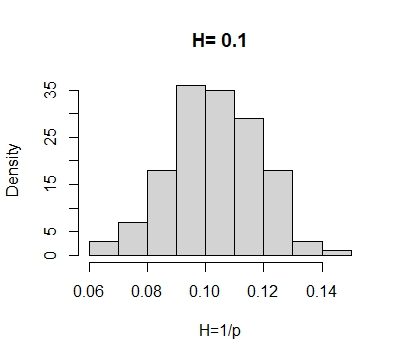
\includegraphics[width=\linewidth]{hist_H01.jpeg}
    \end{subfigure}
    \hfill
    \begin{subfigure}{0.48\textwidth}
        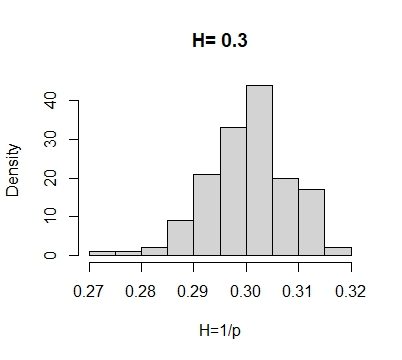
\includegraphics[width=\linewidth]{hist_H03.jpeg}
    \end{subfigure}
    \vskip 0em
    \begin{subfigure}{0.48\textwidth}
        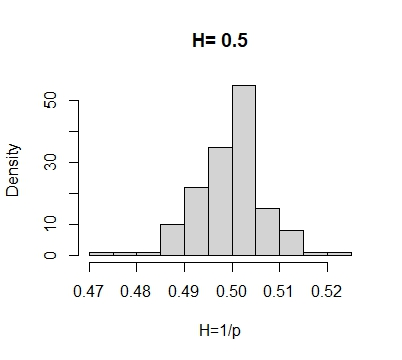
\includegraphics[width=\linewidth]{hist_H05.jpeg}
    \end{subfigure}
    \hfill
    \begin{subfigure}{0.48\textwidth}
        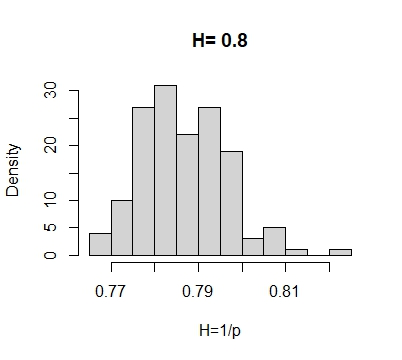
\includegraphics[width=\linewidth]{hist_H08.jpeg}
    \end{subfigure}
    
    \caption{Histogram of estimated roughness index $\hat{H}_{L,K}$ with $L=300\times 300$ and $K=300$ generated from 150 independent simulation of fractional Brownian motions with Hurst parameter $H=\{0.1,0.3,0.5,0.8\}$. }
    \label{fig:checkhist}
\end{figure}\\
In Figure \ref{fig:check2000} we have used $L=2000\times 2000$ and $K=2000$ to make similar plots to those in Figure \ref{fig:checkw} and Figure \ref{fig:checkhist} for a fractional Brownian motion with Hurst parameter $H=0.1$. Table \ref{tab:check2000} provides the summary statistics for the estimated roughness index $\hat{H}_{L,K}$ corresponding to the histogram in Figure \ref{fig:check2000}. We observe that the results are similar to those we obtained for $L=300\times 300$ and $K=300$ but that the estimated roughness index $\hat{H}_{L,K}$ seems to be even more accurate as seen in Figure \ref{fig:check2000} and Table \ref{tab:check2000}. This is not surprising since we know that the normalized $p$-th variation statistic converges to the normalized $p$-th variation as $L$ and $K$ increase. However, increasing $L$ and $K$ is also computationally more demanding. The accuracy of $\hat{H}_{L,K}$ when using $L=300\times 300$ and $K=300$ is satisfactory for many of our purposes. Therefore, we will be using at least $L=300\times 300$ and $K=300$ for the remainder of the thesis.
\begin{table}[htbp]
    \centering
    \begin{tabular}{ccccccc}
        \toprule
        H & Min. & Lower quartile & Median & Mean & Upper quartile & Max. \\
        \midrule
        0.1 & 0.0892 & 0.0963 & 0.0996 & 0.0998 & 0.1031 & 0.1145 \\
        \bottomrule
    \end{tabular}
    \caption{Summary of statistics for estimated roughness index $\hat{H}_{L,K}$ from 150 independent simulations of fBm with $H=0.1$, $L=2000\times 2000$ and $K=2000$.}
    \label{tab:check2000}
\end{table}
\begin{figure}[htbp]
    \centering
    
    \begin{subfigure}{0.48\textwidth}
        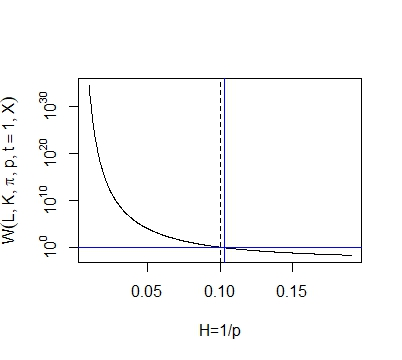
\includegraphics[width=\linewidth]{H01_2000_1.jpeg}
    \end{subfigure}
    \hfill
    \begin{subfigure}{0.48\textwidth}
        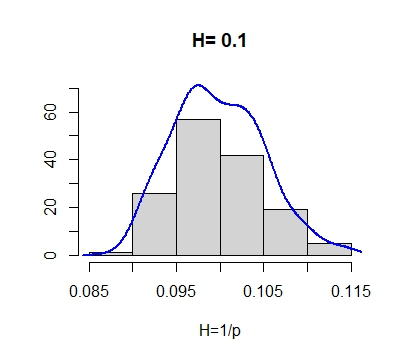
\includegraphics[width=\linewidth]{H01_2000_2.jpeg}
    \end{subfigure}
    
    \caption{Simulation results for fractional Brownian motion with Hurst parameter $H=0.1$. \textbf{Left:} The value of $\log(W(L=2000\times 2000, K=2000, \pi, p, t=1, X=B^H))$ plotted against $H=1/p$ in black. The blue vertical line represents the estimated roughness $\hat{H}_{L,K}$ using $L=2000\times 2000$ and $K=2000$. The vertical black dotted line represents the true Hurst parameter. \textbf{Right:} Histogram of estimated roughness index $\hat{H}_{L,K}$ using $L=2000\times 2000$ and $K=2000$ generated by 150 independent simulations of fBm with Hurst parameter $H=0.1$. The blue line represents a kernel estimator for density. }
    \label{fig:check2000}
\end{figure}\\
We further investigate how the choice of $K<<L$ affects the estimated roughness index $\hat{H}_{L,K}$. In Figure \ref{fig:checkk}, we have plotted the estimated roughness $\hat{H}_{300\times 300,K}$ for a fractional Brownian motion with Hurst parameter $H=0.1$ for different values of $K$ with a fixed $L=300\times 300$. Note that when $\frac{L}{K}$ is not an integer, the $K$ many groups from the definition of normalized $p$-th variation statistic (13) do not contain exactly $\frac{L}{K}$ consecutive points. The code is implemented such that each group will contain either $\lceil \frac{L}{K} \rceil$ or $\lfloor \frac{L}{K} \rfloor$ consecutive points. Figure \ref{fig:checkk} shows that when $K$ is too low, the estimator $\hat{H}_{300\times 300,K}$ seems to be underestimating the true Hurst parameter whereas when $K$ is too high the Hurst parameter is overestimated. For $K\approx \sqrt{L}$ the estimated roughness index is quite consistent and close to the true Hurst parameter $H=0.1$. It is thus natural to use $K=\sqrt{L}$ since $\frac{L}{K}$ will be an integer and the estimator $\hat{H}_{L,K}$ seems to be accurate and consistent in that range.
\begin{figure}[htbp]
    \centering
    
    \begin{subfigure}{0.78\textwidth}
        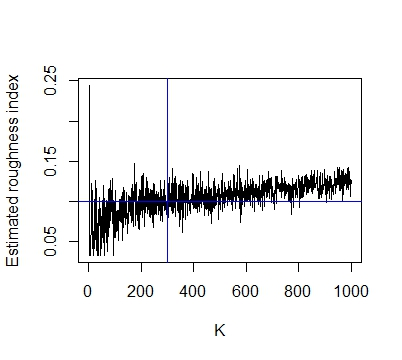
\includegraphics[width=\linewidth]{differentK.jpeg}
    \end{subfigure}
    
    \caption{The solid black line represents the estimated roughness index $\hat{H}_{300\times 300,K}$ plotted against different values of $K$ for a simulation from a fBm with Hurst parameter $H=0.1$. The blue vertical line represents $K=\sqrt{L}=300$ whereas the blue horizontal line represents the true Hurst parameter $H=0.1$.}
    \label{fig:checkk}
\end{figure}\\

\subsection{Instantaneous volatility and realized volatility}
As mentioned in (1) log-prices are often modelled as continuous semi-martingales where the derivative of the log-price $Y_t$ takes the form
\begin{align*}
dY_t = \mu_tdt+\sigma_tdW_t.
\end{align*}
The term $\sigma_t$ represents the volatility process, and $\sigma_t$ is also called instantaneous volatility or spot volatility. In stochastic volatility models, $\sigma_t$ is represented as a stochastic process itself often driven by a fractional process. Contrary to prices of an asset, instantaneous volatility cannot be directly observed and needs to be estimated from prices.\\
In a practical situation, the price of the asset $S_t$ at time $t$ is usually observed over a non-uniform time grid of $[0,T]$:
\begin{align*}
\pi^n = \left(0=t^n_0<t^n_1<...<t^n_{N(\pi^n)}=T\right).
\end{align*}
For high-frequency data the assumption (12) is often assumed. That is, $\rvert \pi^n\lvert\rightarrow 0$ as $n$ increases where $n$ can be thought of as a sampling frequency i.e. the number of samples per second (or per other unit).\\\\
For $Y_t= \log(S_t)$ the instantaneous volatility $\sigma_t$ can be recovered by 
\begin{align*}
\sigma_t^2 =  \frac{d}{dt} \lim_{n\rightarrow \infty} \sum_{\pi^n \cap [0,t]} \left( Y(t_{i+1}^n)-Y(t_i^n)\right)^2 = \lim_{n\rightarrow \infty} RV_t^2(\pi^n)^2
\end{align*} 
where the realized variance along the sampling grid $\pi^n$ is defined as
\begin{align}
RV_t(\pi^n)^2 = \sum_{\pi^n \cap [0,t]}\left(Y(t_{i+1}^n )-Y(t_i^n)\right)^2. \label{eq:reavardef}
\end{align} 
The realized volatility over time interval $[t,t+\Delta]$ along the sampling grid $\pi^n$ is then defined as 
\begin{align}
RV_{t,t+\delta}(\pi^n) = \sqrt{\sum_{\pi^n \cap [t,t+\Delta]}\left(Y(t_{i+1}^n )-Y(t_i^n)\right)^2}. \label{eq:rvdef}
\end{align}
If the price $S_t$ follows a stochastic volatility model as, it is known that the realized variance converges to the quadratic variation of $Y$ as sampling frequency increases (Jacod and Protter)
\begin{align*}
 RV_{t,t+\Delta} (\pi^n) \overset{\mathbb{P}}{\underset{n \to \infty}{\longrightarrow}} \sqrt{\int^{t+\Delta}_t\sigma^2_u du}.
\end{align*}
Hence, along a single price path observed at high-frequency, we can compute the realized volatility \eqref{eq:rvdef} and use this as an indicator of volatility
\begin{align*}
 RV_{t,t+\Delta} (\pi^n)\simeq \sqrt{\Delta} \sigma_t.
\end{align*}
As $n$ increases the estimation becomes more accurate \cite{cont}.

\subsection{Smoothness of a path by logarithmic regression} 
In this section we will introduce the smoothness estimator via logarithmic regression used in \cite{gatheral}. Consider a volatility process on a time grid $[0,T]$. First we pretend that we have access to discrete observations of the spot volatility process with mesh $\Delta$ such that the observations are $\sigma_0, \sigma_\Delta, ..., \sigma_{k\Delta},...$ for $k \in \{0, \lfloor T / \Delta \rfloor\}$. Here $\Delta$ is a natural number and $\Delta\geq 1$. If we set $N=\lfloor T / \Delta \rfloor$, then for $q\geq 0$ we define
\begin{align*}
m(q,\Delta) = \frac{1}{N} \sum_{k=1}^N \lvert \log(\sigma_{k\Delta})-\log(\sigma_{(k-1)\Delta})\rvert^q.
\end{align*}
Following \cite{gatheral} the main assumption is that for some $s_q>0$ and $b_q>0$
\begin{align}
N^{qs_q}m(q,\Delta)\to b_q
\end{align}
as $\Delta$ tends to zero. Under additional technical assumptions, this essentially means that the volatility process belongs to a Besov smoothness space $\mathcal{B}^{s_q}_{q,\infty}$ and does not belong to $\mathcal{B}^{s_q'}_{q,\infty}$ for $s_q'>s_q$. Hence, $s_q$ can be considered as a smoothness parameter. In particular, if $\log(\sigma_t)$ is a fractional Brownian motion with Hurts parameter $H$, then for any $q\geq 0$  equation (17) holds in probability with $s_q=H$. It can further be shown that the sample paths of the process do indeed belong to $\mathcal{B}^{s_q}_{q,\infty}$. Thus, $s_q$ is a measure of the smoothness (or roughness) of the volatility process \cite{gatheral}.\\\\
The instantaneous volatility can not be directly observed, and exact computations of $m(q,\Delta)$ is not possible in practice.  In order to make use of $m(q,\Delta)$ we must therefore approximate the true spot volatility. The estimated volatility can be computed by the realized volatility or some variation of realized volatility. In the following we will be using the notation $m(q, \Delta)$ with the understanding that we are only approximating the true spot volatility. To estimate the smoothness parameter $s_q$ for each $q$, we can compute $m(q,\Delta)$ for different values of $\Delta$ and regress $\log m(q,\Delta)$ against $\log \Delta$. Note that for a given $\Delta$ several $m(q,\Delta)$ can be computed depending on the starting point. For example, if $\Delta=3$ then the starting point can be $\hat{\sigma}_0$, $\hat{\sigma}_{\Delta}$ or $\hat{\sigma}_{2\Delta}$. The final measure of $m(q,\Delta)$ is computed as the average of these values of $m(q,\Delta)$ with different starting points.\\\\
\cite{gatheral} shows that for a given $q$, $\log m(q,\Delta)$ values regressed against $\log \Delta$ essentially lie on a straight line. Assuming stationary increments of the log-volatility, this implies that the increments fulfil the scaling property 
\begin{align*}
\mathbb{E}\left[ \lvert \log (\sigma_\Delta) - \log (\sigma_0) \rvert^q\right] = b_q\Delta^{\zeta _q}
\end{align*}
where $\zeta_q = qs_q>0$ is the slope of the line associated to $q$. This result uses that $m(q,\Delta)$ can be seen as the empirical counterpart of $\mathbb{E}\left[ \lvert \log (\sigma_\Delta) - \log (\sigma_0) \rvert^q\right]$. Furthermore, \cite{gatheral} shows that $s_q$ seems to not depend on $q$, and plotting $\zeta_q$ against $q$ shows $\zeta_q \sim qs_q$.\\\\
Thus, we can compute an estimate of the smoothness (or roughness) of a volatility process by first regressing $\log m(q,\Delta)$ against $\log \Delta$ for different values of $q$. The slope of the straight line is an estimate of $\zeta_q$. Next, we regress $\zeta_q$ against $q$. The slope of the straight line is and estimate of the smoothness parameter $s_q$. If $\log(\sigma_t)$ is a fractional Brownian motion then $s_q=H$ holds in probability where $H$ is the Hurst parameter.\\\\
In Figure \ref{fig:oxfordlog} we have replicated the method used in \cite{gatheral} to estimate the roughness index of the volatility of S\&P500 using the first 3500 days of the daily realized variance estimates from the Oxford-Man Institute of Quantitative Finance Realized Library for S\&P. Our results coincide with the results from \cite{gatheral}, and the log-regression yields a straight line for all our values of $q$. Our estimated smoothness of the S\&P500 volatility is $H=0.1421$.
\begin{figure}[htbp]
    \centering
    
    \begin{subfigure}{0.48\textwidth}
        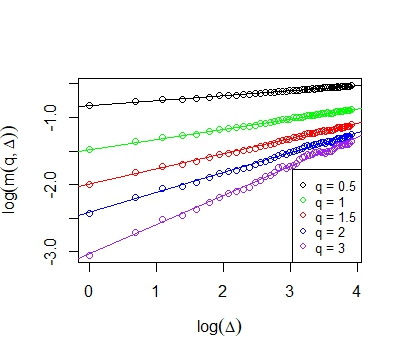
\includegraphics[width=\linewidth]{volis1.jpeg}
    \end{subfigure}
    \hfill
    \begin{subfigure}{0.48\textwidth}
        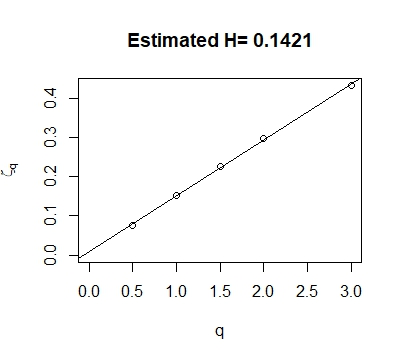
\includegraphics[width=\linewidth]{volis2.jpeg}
    \end{subfigure}
    
    \caption{A reproduction of the log-regression method introduced by \cite{gatheral} using the first 3500 days of the daily realized variance estimates from the Oxford-Man Institute of Quantitative Finance Realized Library for S\&P. The estimated roughness is $H=0.1421$. }
    \label{fig:oxfordlog}
\end{figure}\\
In Figure \ref{fig:oxfordw} we have used the roughness estimator from section 3.1 on the same S\&P500 volatility data to estimate the roughness. We have used $W(L = 3500, K = \sqrt{3500}, \pi, p, t=1, X)$ since the dataset only consist of 3500 days. We have set $t=1$ since $t$ simply works as a scaling parameter. The conclusions are the same for $t=1$ as for $t=3500$. The estimated roughness index is $\hat{H}_{L,K}=0.1425$. We immediately observe that the estimated roughness index is very close to the estimated smoothness parameter from the log-regression method $s_q=0.1421$. However, note that $L=3500$ is much smaller than $L=300\times 300 = 90000$ for which we have investigated the accuracy of the roughness estimator via normalized $p$-th variation statistic. Therefore, the estimated roughness estimator $\hat{H}_{L,K}$ might not be very precise. The results do however indicate that our two different approaches to estimate the roughness of a volatility process coincides.
\begin{figure}[htbp]
    \centering
    
    \begin{subfigure}{0.78\textwidth}
        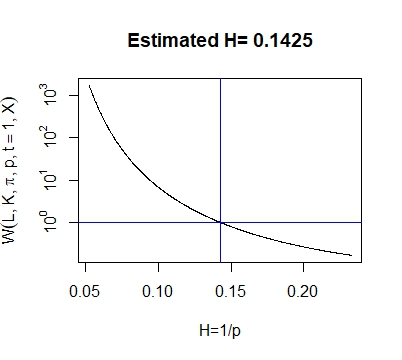
\includegraphics[width=\linewidth]{volisW.jpeg}
    \end{subfigure}
    
    \caption{Estimating the roughness of the first 3500 days of S\&P500 volatility data from Oxford-Man Institute of Quantitative Finance Realized Library using the roughness estimator from section 3.1 with $L=3500$ and $K=\sqrt{3500}$. The estimated roughness index is $\hat{H}_{L,K}=0.1425$.}
    \label{fig:oxfordw}
\end{figure}\\

\subsection{Sequential scale estimator of roughness exponent}
The third estimator we will introduce, is the sequential scale estimator of roughness first introduced by \cite{han}. This estimator differs from many other roughness estimators by the fact that it is computed directly from discrete observations of realized variance. That is, the input to the estimator needs to be realized variance and not instantaneous variance or volatility. The two previously described estimators are based on having access to discrete observations of instantaneous volatility $\sigma_t$. Realized volatility is then used as an approximation of the true spot volatility. This two step approach can be problematic since the estimation error in the realized volatility might substantially distort the outcome of the final roughness estimation. The sequential scale estimator avoids these possible inaccuracies caused by the estimation errors since it is based directly on realized variance.\\\\
\cite{han} are mainly concerned with stochastic volatility models based on fractional Brownian motions, but many aspects of the approach works in a model-free setting. Let $x: [0,1] \rightarrow \mathbb{R}$ be any continuous function. For $p\geq 1$ the $p$-th variation of the function $x$ along the $n$-th dyadic partition is defined as
\begin{align*}
\langle x \rangle^{(p)}_n := \sum_{k=0}^{2^n-1} \lvert x((k+1)2^{-n})-x(k2^{-n})\rvert^p.
\end{align*}
The above definition is similar to Definition 1. If there exist a $R\in [0,1]$ such that
\begin{align*}
\lim_{n\rightarrow\infty}\langle x \rangle^{(p)}_n =
\begin{cases} 
0 & \text{for } p > \frac{1}{R} \\
\infty & \text{for } p < \frac{1}{R}
\end{cases}
\end{align*}
we refer to $R$ as the roughness exponent of $x$. The smaller $R$ the rougher is the path $x$ and vice verse. Moreover, if $x$ is a sample path of a fractional Brownian motion, the roughness exponent R is equal to the Hurst parameter $H$ \cite{han}.\\\\
Now, since only asset prices and their realized variance can be observed in practice, we can consider this as making discrete observations of
\begin{align}
y(t) = \int_0^t g\left(x(s)\right) ds, \quad 0\leq t \leq 1, \label{eq:intvar}
\end{align}
where $g: \mathbb{R}\rightarrow \mathbb{R}$ is sufficiently regular. Here $y(t)$ shall be seen as integrated variance. Therefore, $g(x(t))$ should represent the variance of the underlying model. For instance, if log-volatility is given by a fractional Ornstein-Uhlenbeck process, we will take $x$  as a sample path of a fractional Ornstein-Uhlenbeck process and $g(t)=(e^t)^2 = e^{2t}$.\\\\
For the estimator, it is supposed that for a given $n\in \mathbb{N}$ we have access to the discrete observations $\{y(k2^{-n-2}):k=0,...,2^{n+2}\}$ of the integrated variance (i.e. the function $y$ in (\ref{eq:intvar})). Based on these data points, the following coefficients are introduced
\begin{align}
\vartheta_{n,k} := 2^{3n/2+3} \left( 
y\left( \frac{4k}{2^{n+2}} \right) 
- 2y\left( \frac{4k+1}{2^{n+2}} \right) 
+ 2y\left( \frac{4k+3}{2^{n+2}} \right) 
- y\left( \frac{4k+4}{2^{n+2}} \right) 
\right),
\end{align}
for $0\leq k \leq 2^n - 1$. The estimator for the roughness exponent is then given by
\begin{align*}
\hat{\mathscr{R}}_n (y) := 1 - \frac{1}{n}\log_2 \sqrt{\sum_{k=0}^{2^n-1}\vartheta_{n,k}^2}.
\end{align*}
Detailed explanation of the rationale behind the estimator can be seen in \cite{han} where convergence and consistency results are also shown.\\\\
The estimator $\hat{\mathscr{R}}_n (y)$ is not scale-invariant, and \cite{han} suggest to do scale-invariant modifications of $\hat{\mathscr{R}}_n (y)$. Fix $m\in \mathbb{N}$ with $n>m$ and fix $\alpha_0, ..., \alpha_m \geq 0$ with $\alpha_0>0$. The sequential scaling factor $\lambda_n^s$ is then defined as
\begin{align}
\lambda_n^s := \arg\min_{\lambda>0} \sum_{k=n-m}^n \alpha_{n-k} \left( \hat{\mathscr{R}}_k (\lambda y)-\hat{\mathscr{R}}_{k-1} (\lambda y)\right)^2 . \label{eq:scale_lambda}
\end{align}
The sequential scaling estimate $\hat{\mathscr{R}}_n^s (y)$ is then defined as follows 
\begin{align*}
\hat{\mathscr{R}}_n^s (y) := \hat{\mathscr{R}}_n (\lambda_n^s y).
\end{align*}
The idea is that the sequential scaling factor $\lambda_n^s$ enforces the convergence of $\hat{\mathscr{R}}_n (\lambda_n^s y)$. Thus, $\hat{\mathscr{R}}_n^s (y)$ will in some cases converge faster than $\hat{\mathscr{R}}_n (y)$ and remove bias. \cite{han} prove that the sequential scale estimator is scale-invariant and has a unique solution for every function $y\in C[0,1]$.\\\\
In practice the roughness exponent is usually estimated from realized variance rather than integrated variance. That is, realized variance is used as an approximation of integrated variance. Let $(m_n)_{n\in \mathbb{N}_0}$ be a fixed increasing sequence, where $m_n$ can be regarded as the number of observed data points used to compute the realized variance over each interval $[k2^{-n},(k+1)2^{-n}]$. Then we can denote the realized variance used for the sequential scale estimator in the following way
\begin{align}
\widehat{Y}_t^{(n)} := \sum_{k=1}^{\lfloor 2^nm_nt \rfloor} \left( \log S_{\frac{k}{2^n m_n}} - \log S_{\frac{k-1}{2^n m_n}}\right)^2 . \label{eq:rvforscale}
\end{align}
Thus, the process $\widehat{Y}_t^{(n)}$ is the realized variance calculated from the price process $S_t$ with a mesh size $(2^nm_n)^{-1}$. From $\widehat{Y}_t^{(n)}$ we can define the proxy coefficients $\widetilde{\vartheta}_{n,k}$ as
\begin{align*}
\widetilde{\vartheta}_{n,k} := 2^{3n/2+3} \left( 
\widehat{Y}_{ \frac{4k}{2^{n+2}}}^{(n+2)}
- 2\widehat{Y}_{\frac{4k+1}{2^{n+2}}}^{(n+2)}
+ 2\widehat{Y}_{\frac{4k+3}{2^{n+2}}}^{(n+2)} 
- \widehat{Y}_{\frac{4k+4}{2^{n+2}}}^{(n+2)} 
\right).
\end{align*}
By replacing $\vartheta_{n,k}$ with $\widetilde{\vartheta}_{n,k}$ we can construct an estimator $\widetilde{\mathscr{R}}_n (y)$ that directly estimates the roughness exponent from the realized variance as follows
\begin{align*}
\widetilde{\mathscr{R}}_n (S) := 1 - \frac{1}{n}\log_2 \sqrt{\sum_{k=0}^{2^n-1}\widetilde{\vartheta}_{n,k}^2}
\end{align*}
where $S$ denotes the price process that $\widetilde{\mathscr{R}}_n$ estimates from. \cite{han} show that under certain assumptions on the difference between $\widehat{Y}_t^{(n)}$ and $Y_t^{(n)}$, then $\widetilde{\mathscr{R}}_n (S)$ and $\hat{\mathscr{R}}_n (Y)$ converge to the same limit as $n$ increases provided that $m_n$ grows fast enough. We will by $\widetilde{\mathscr{R}}_n^s (S)$ denote the sequential scale estimator of realized variance which is defined as
\begin{align*}
\widetilde{\mathscr{R}}_n^s (\widehat{Y}_t^{(n)}) := \widetilde{\mathscr{R}}_n (\lambda_n^s \widehat{Y}_t^{(n)})
\end{align*} 
where $\lambda_n^s$ is computed in the same manner as (\ref{eq:scale_lambda}) just using $\widetilde{\mathscr{R}}_n(\widehat{Y}_t^{(n)})$ instead of $\widehat{\mathscr{R}}_n(Y)$.\\\\
We will now illustrate the performance of $\hat{\mathscr{R}}_n^s (y)$ and $\hat{\mathscr{R}}_n (y)$ in a simple example by replicating a simulation example from \cite{han}. We let $x$ follow a sample path of a fractional Brownian motion $W^H_t$ and set $g(x)=x$. For the computation of $\hat{\mathscr{R}}_n (y)$ we require observations of $y$ at all values of the time grid $\mathbb{T}_{n+2}:= \{k 2^{-n-2} : k=0,1,...,2^{n+2}\}$. In order to approximate $y(t)=\int_0^t W^H_s ds$ we are simulating the values of $W^H_t$ on a finer time grid $\mathbb{T}_N$ with $N=n+6$. Then we put
\begin{align}
Y_{k2^{-n-2}}:= 2^{-N} \sum_{j=1}^{2^{N-n-2}k} W^H_{j2^{-N}}, \quad k=0,1,...,2^{n+2} \label{eq:scaley}
\end{align}
which is an approximation of $y(t)=\int_0^t W^H_s ds$ by Riemann sums. In Figure \ref{fig:scaleplot} we display the results for the estimators $\hat{\mathscr{R}}_n (y)$ and $\hat{\mathscr{R}}_n^s (y)$ for 1000 independent paths of a fractional Brownian motion for different values of $n$. The left plot of Figure \ref{fig:scaleplot} is based on paths from a fractional Brownian motion with Hurst exponent $H=0.3$ while the right plot is for a fBm with $H=0.7$. The top plots are from the original estimator $\hat{\mathscr{R}}_n (y)$ whereas the bottom plots are box plots of the sequential scale estimates $\hat{\mathscr{R}}_n^s (y)$. We observe from the top plots in Figure \ref{fig:scaleplot} that $\hat{\mathscr{R}}_n (y)$ performs relatively well and seems to converge to the true roughness exponent as $n$ increases. However, the estimator also exhibits a certain bias. The corresponding results for the sequential scale estimator $\hat{\mathscr{R}}_n^s (y)$ are displayed in the bottom plots of Figure \ref{fig:scaleplot}. We observe that by passing to the sequential scale estimator we completely remove the bias observed for $\hat{\mathscr{R}}_n (y)$. Overall, $\hat{\mathscr{R}}_n^s (y)$ seems to be performing very well especially for $n\geq 15$. We will be using the sequential scaling estimate $\hat{\mathscr{R}}_n^s (y)$ with $n\geq 15$ when performing numerical experiments in section 4.
\begin{figure}[htbp]
    \centering
    
    \begin{subfigure}{0.48\textwidth}
        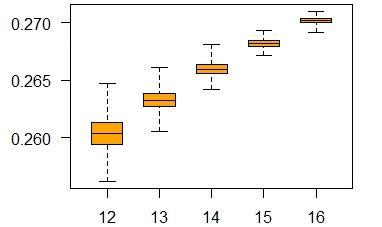
\includegraphics[width=\linewidth]{box3.png}
    \end{subfigure}
    \hfill
    \begin{subfigure}{0.48\textwidth}
        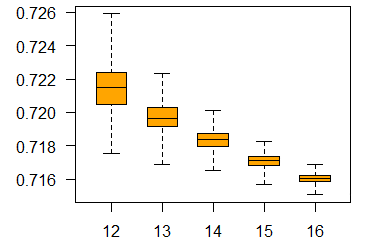
\includegraphics[width=\linewidth]{box1.png}
    \end{subfigure}
    \vskip 0em
    \begin{subfigure}{0.48\textwidth}
        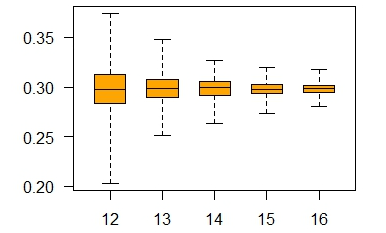
\includegraphics[width=\linewidth]{box4.png}
    \end{subfigure}
    \hfill
    \begin{subfigure}{0.48\textwidth}
        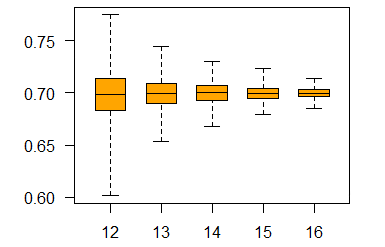
\includegraphics[width=\linewidth]{box2.png}
    \end{subfigure}
    
    \caption{Box plots of the original estimates $\hat{\mathscr{R}}_n (y)$ (top) and the sequential scale estimates $\hat{\mathscr{R}}_n^s (y)$ (bottom) for $n=12,...,16$ based on 1000 independent simulations of a fractional Brownian motion with $H=0.3$ (left) and $H=0.7$ (right) and with $Y$ as in (\ref{eq:scaley}). The other parameters are chosen to be $m=3$ and $\alpha_k = 1$ for $k=0,1,2,3$.} \label{fig:scaleplot}
\end{figure}\\

\section{Numerical Experiments}
In this section we will be performing a number of numerical experiments. We will be estimating the roughness index for stochastic models based directly on the instantaneous volatility $\sigma_t$ and based on the realized volatility by using price trajectories simulated from the models. By doing this we can investigate how estimation errors impact the estimated roughness index. We will be performing these experiments for stochastic models with various degrees of roughness.

\subsection{Simple stochastic volatility diffusion model}
First, we will consider the following stochastic volatility model where the volatility is the modulus of a Brownian motion:
\begin{align}
dS_t = \sigma_t S_t dB_t \quad \text{with} \quad \sigma_t = \lvert W_t \rvert, \label{eq:simple}
\end{align}
where $S_t$ is the price of the asset and $B_t$ and $W_t$ are two independent Brownian motions. For the simulation we use $S_0=1$ and $T=1$. The true roughness of this model is simply $H=0.5$.\\\\
We are estimating the realized variance using \eqref{eq:rvdef} for 300 consecutive points which corresponds to a 5 minute moving window when the price is updated every second. We estimate the roughness of the volatility process by using the realized volatility and instantaneous volatility as data in our roughness estimators. For every 300 consecutive points we are computing the realized volatility $RV_{t,t+\delta}(\pi^n)$ as in \eqref{eq:rvdef} and rescale the volatility to represents the same time interval as the corresponding instantaneous volatility $\sigma_t$. The corresponding instantaneous volatility is then the $\sigma_t$ for the first of these 300 points. In Figure \ref{fig:ex5IVRV}, we have made plots for the realized and instantaneous volatility. The left plot of Figure \ref{fig:ex5IVRV} represents the realized volatility of the price process in black and the instantaneous volatility in red. The middle plot of Figure \ref{fig:ex5IVRV} represents the difference between the realized and instantaneous volatility which is the estimation error. The right plot of Figure \ref{fig:ex5IVRV} represents the log difference between the realized and instantaneous volatility. Figure \ref{fig:ex5IVRV} indicates that the estimation error has a complicated dependence structure. There seems to be no obvious pattern in the estimation error and both the estimation error and log estimation error are far from I.I.D. 
\begin{figure}[h]
    \centering
    \begin{subfigure}{0.32\textwidth}
        \centering
        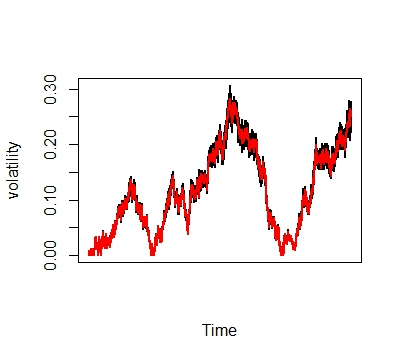
\includegraphics[width=\textwidth]{ex5_IVRV1.jpeg}
    \end{subfigure}\hfill
    \begin{subfigure}{0.32\textwidth}
        \centering
        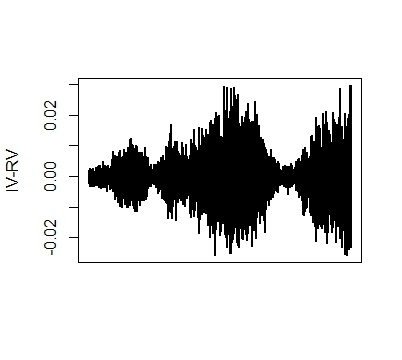
\includegraphics[width=\textwidth]{ex5_IVRV2.jpeg}
    \end{subfigure}\hfill
    \begin{subfigure}{0.32\textwidth}
        \centering
        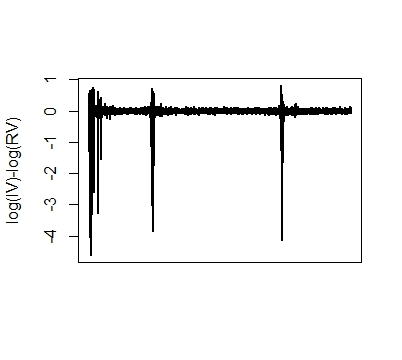
\includegraphics[width=\textwidth]{ex5_IVRV3.jpeg}
    \end{subfigure}
    \caption{Simulation from model \eqref{eq:simple}. \textbf{Left:} The red line represents instantaneous volatility $\sigma_t$ whereas the black line represents realized volatility $RV_t$. \textbf{Middle:} Corresponding estimation error for the left simulated path. \textbf{Right:} Corresponding log estimation error.}
    \label{fig:ex5IVRV}
\end{figure}\\\\
In Figure \ref{fig:ex5w} we have estimated the roughness index via normalized $p$-th variation from section 3.1 for realized and instantaneous volatility. In the left plot, we have used the realized volatility as data in the normalized $p$-th variation statistic and plotted $\log(W(K=500, L= 500\times 500, \pi, p, t=1, X = RV))$ against $H=\frac{1}{p}$. The right graph is a similar plot using instantaneous volatility instead of realized volatility. The obtained roughness estimators are very different for instantaneous and realized volatility. For realized volatility we obtain an estimated roughness of $\hat{H}_{L=500\times 500, K=500}(RV)=0.323$ which is much lower than the estimated roughness index for instantaneous volatility $\hat{H}_{L=500\times 500, K=500}(\sigma)=0.499$. The true roughness of the model is $H=0.5$. Thus, the roughness estimator is quite accurate when using instantaneous volatility which is in accordance with our results from section 3. However, the estimated roughness when using realized volatility is much rougher than the true roughness. As this is a simulation study we do have any measurement errors, and this rougher behaviour of realized volatility purely comes from the estimation error.
\begin{figure}[htbp]
    \centering
    
    \begin{subfigure}{0.48\textwidth}
        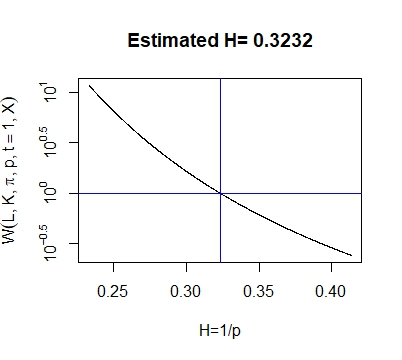
\includegraphics[width=\linewidth]{ex5_RVw.jpeg}
    \end{subfigure}
    \hfill
    \begin{subfigure}{0.48\textwidth}
        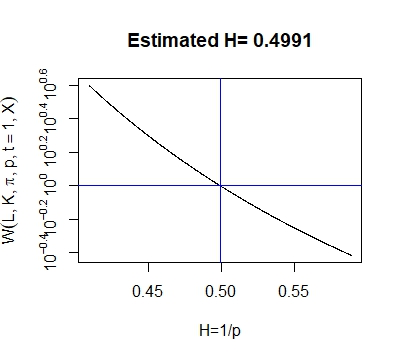
\includegraphics[width=\linewidth]{ex5_IVw.jpeg}
    \end{subfigure}
    
    \caption{The value of $\log(W(L=500\times 500, K=500, \pi, p, t=1, X))$ plotted against $H=1/p$ in black. The blue vertical line represents the estimated roughness $\hat{H}_{L,K}$. \textbf{Left:} Estimated roughness index $\hat{H}_{L,K}$ for realized volatility derived from the stochastic volatility model \eqref{eq:simple}. \textbf{Right:} Estimated roughness index for instantaneous volatility of the same price path.}
    \label{fig:ex5w}
\end{figure}\\\\
In Figure \ref{fig:ex5k} we have plotted the estimated roughness index $\hat{H}_{L=500\times 500,K}$ against different values of $K$. The left graph is for realized volatility while the right graph is for instantaneous volatility. The blue lines represents the estimated roughness $\hat{H}_{L,K}$ with $L=500\times 500$ and $K=500$ which are also reported in Figure \ref{fig:ex5w}. From the figure, we observe that irrespective of the choice of $K$ for the finite sample dataset of length $L=500\times 500$, the realized volatility is significantly rougher than the instantaneous volatility. The estimated roughness of the volatilities are quite consistent as long as $K$ is not too low for both volatilities. However, $\hat{H}_{L=500\times 500,K}$ seems to be even more consistent for instantaneous volatility than for the realized volatility.
\begin{figure}[htbp]
    \centering
    
    \begin{subfigure}{0.48\textwidth}
        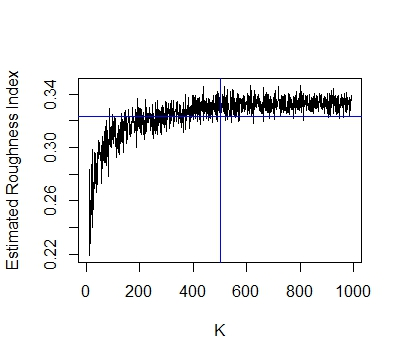
\includegraphics[width=\linewidth]{ex5_RVk.jpeg}
    \end{subfigure}
    \hfill
    \begin{subfigure}{0.48\textwidth}
        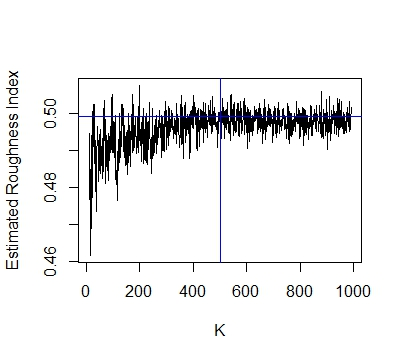
\includegraphics[width=\linewidth]{ex5_IVk.jpeg}
    \end{subfigure}
    
    \caption{The value of the estimated roughness index $\hat{H}_{L = 500\times 500 ,K}$ plotted against different values of $K$. \textbf{Left:} Estimated roughness index $\hat{H}_{L= 500\times 500,K}$ for realized volatility derived from the stochastic volatility model \eqref{eq:simple}. The horizontal blue line represents $\hat{H}_{L=500\times 500,K = 500} = 0.323$. \textbf{Right:} Estimated roughness index for instantaneous volatility of the same price path. The horizontal blue line represents $\hat{H}_{L=500\times 500,K = 500} = 0.499$.}
    \label{fig:ex5k}
\end{figure}\\\\
We now want to use the sequential scale estimator $\hat{\mathscr{R}}_n^s (y)$ to estimate the roughness for the same path that Figure \ref{fig:ex5w} was based on. The sequential scale estimator requires observations of integrated or realized variance $y(t) = \int_0^t g\left(x(s)\right) ds$ at all values of the time grid $\mathbb{T}_{n+2}:= \{k 2^{-n-2} : k=0,1,...,2^{n+2}\}$. To accommodate for that we rescale our simulated path from before. We will use $n=17$ for the roughness estimation. Now, to approximate $y$ properly we set $m_{17} = 2^5 = 32$ which is the number of data points in each interval $[k2^{-n},(k+1)2^{-n}]$. We then follow the procedure described in section 3.5 and make sure that we have values of the price process on the finer time grid $\mathbb{T}_{N}$ with $N=n+7$. Therefore, we need $2^N+1$ points on the time interval $t\in[0,1]$. Thus, for these points we have $\Delta t = 2^{-N}$. We rescale the first $2^N$ points of our simulated Brownian motions $B_t$ and $W_t$ such that they correspond to this new $\Delta t$. We then generate the price process as in (\ref{eq:simple}) using these rescaled Brownian motions. In Figure \ref{fig:ex5price} we have plotted the first 100000 data points of the original price process $S_t$ on the left and the corresponding rescaled price process on the right. We observe that the prices processes follow the exact same pattern. The only difference between the graphs is the axes that have been rescaled since we have rescaled the whole prices process. Therefore, we would expect the same roughness index of the two price processes. 
\begin{figure}[htbp]
    \centering
    
    \begin{subfigure}{0.48\textwidth}
        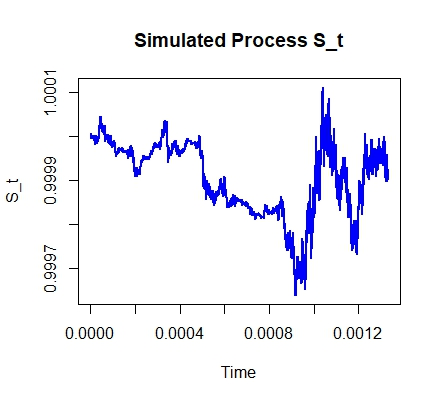
\includegraphics[width=\linewidth]{price_plot.jpeg}
    \end{subfigure}
    \hfill
    \begin{subfigure}{0.48\textwidth}
        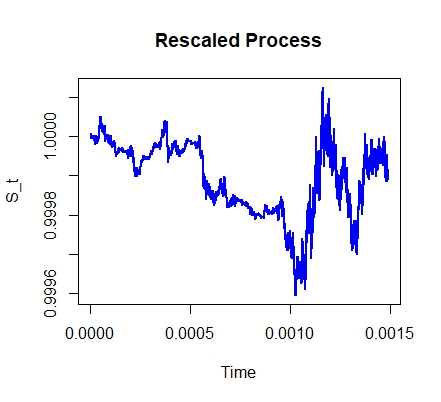
\includegraphics[width=\linewidth]{price_rescaled.jpeg}
    \end{subfigure}
    
    \caption{The first 100000 data points of the simulated price process $S_t$ generated from model (\ref{eq:simple}). The left plot is the original simulated path while the right plot is the rescaled price process with fewer points and a different mesh size used for the sequential scale estimator.}
    \label{fig:ex5price}
\end{figure}\\\\
We then compute the realized variance as in (\ref{eq:rvforscale}). In order to compare the realized variance/volatility with instantaneous volatility, we also approximate $y(t) = \int_0^t g\left(x(s)\right) ds$ directly from $\sigma_t$ by 
\begin{align}
Y_{k2^{-n-2}}:= 2^{-N} \sum_{j=1}^{2^{N-n-2}k} \sigma^2_{j2^{-N}}, \quad k=0,1,...,2^{n+2}. \label{eq:ex5y}
\end{align}
In Figure \ref{fig:ex5scale} we have plotted these two approximations of integrated variance $y(t)$ and their difference. The left plot of Figure \ref{fig:ex5scale} represent the realized variance in black and the approximation $Y$ directly from $\sigma_t$ as in (\ref{eq:ex5y}) in red. The middle plot shows the difference between these two approximations of integrated variance, and the right plot shows the difference between the log of the two approximations. Figure \ref{fig:ex5scale} indicates that these two ways of computing the integrated variance yield very similar results, and the difference between realized variance and $Y$ is very small. On the left plot it is difficult to distinguish the red and the black line from each other since they fall directly on top of each other. However, there is a small difference as seen on the two plots to the right, and especially the log difference is quite big in the beginning when the integrated variance is very small. \\
\begin{figure}[h]
    \centering
    \begin{subfigure}{0.32\textwidth}
        \centering
        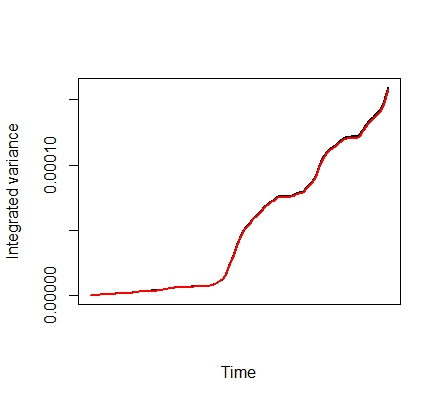
\includegraphics[width=\textwidth]{ex5_scale1.jpeg}
    \end{subfigure}\hfill
    \begin{subfigure}{0.32\textwidth}
        \centering
        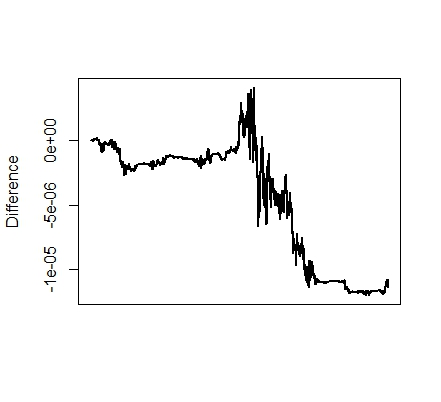
\includegraphics[width=\textwidth]{ex5_scale2.jpeg}
    \end{subfigure}\hfill
    \begin{subfigure}{0.32\textwidth}
        \centering
        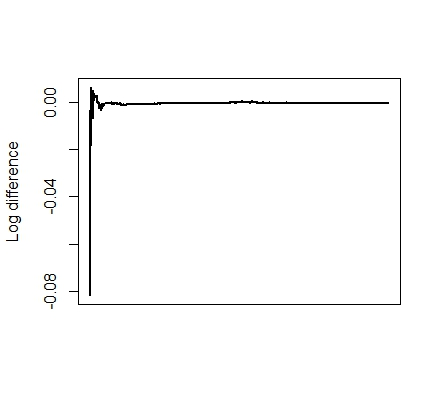
\includegraphics[width=\textwidth]{ex5_scale3.jpeg}
    \end{subfigure}
    \caption{Integrated variance of the original path from model \eqref{eq:simple} rescaled to fit the sequential scale estimator. \textbf{Left:} The red line represents $Y$ computed directly from instantaneous volatility $\sigma_t$ whereas the black line represents realized variance $RV_t^2$. \textbf{Middle:} Corresponding difference between the lines in the left plot. \textbf{Right:} Corresponding log difference.}
    \label{fig:ex5scale}
\end{figure}\\\\
We now proceed to estimating the roughness by using respectively realized variance and spot variance $Y(\sigma_t)$. We denote the sequential scale estimator based directly on realized variance by $\widetilde{\mathscr{R}}_n^s (S)$ whereas the roughness estimated from $Y(\sigma_t)$ is denoted by $\widehat{\mathscr{R}}_n^s (Y)$. Table \ref{tab:ex5scaleest} provides the roughness estimates obtained from the sequential scale estimator for the rescaled path from model (\ref{eq:simple}). Furthermore, the table also provides the results from the original estimators $\widetilde{\mathscr{R}}_n (S)$ and $\widehat{\mathscr{R}}_n (Y)$ that are used for the computations of $\widetilde{\mathscr{R}}_n^s (S)$ and $\widehat{\mathscr{R}}_n^s (Y)$. Even though the difference between realized variance $\widehat{Y}_t^{(n)}$ and $Y(\sigma_t)$ is small, the sequential scale estimator yields very different results when used for these two variances as seen in Table \ref{tab:ex5scaleest}. The estimated roughness when using spot variance $Y(\sigma_t)$ is very close to the true roughness of the model $H=\frac{1}{2}$. However, when using realized variance the estimated roughness is $\widetilde{\mathscr{R}}_n^s (S)=-0.1073$ which is a value that roughness can never take. This indicates that the estimator $\widetilde{\mathscr{R}}_n^s (S)$ is very vulnerable to estimation errors in sense of difference between realized variance and integrated variance. This is surprising since the sequential scale estimator has been developed with the focus of avoiding the problems in roughness estimation caused by estimation errors. It is clear that the estimation error is smaller for the sequential scale estimator in the sense that the difference between realized variance $\widehat{Y}_t^{(n)}$ and $Y(\sigma_t)$ observed in Figure \ref{fig:ex5scale} is much smaller than the difference between realized volatility and instantaneous volatility observed in Figure \ref{fig:ex5IVRV}. However, the small difference between $\widehat{Y}_t^{(n)}$ and $Y(\sigma_t)$ is enough to substantially distort the outcomes of the roughness estimation. Furthermore, we observe from Table \ref{tab:ex5scaleest} that the original estimator $\widetilde{\mathscr{R}}_n(S)$ actually performs better than the sequential scale estimator $\widetilde{\mathscr{R}}_n^s(S)$ when used for realized variance. This is surprising since we illustrated in our simulation examples from section 3.5 how passing to the sequential scale estimator could remove bias and make the estimator converge faster. However, both $\widetilde{\mathscr{R}}_n^s(S)$ and $\widetilde{\mathscr{R}}_n(S)$ performs very poorly in this example.
\begin{table}[htbp]
    \centering
    \begin{tabular}{ccc}
        \toprule
         & Realized variance & Spot variance $Y(\sigma_t)$ \\
        \midrule
        Sequential scale estimator & $\widetilde{\mathscr{R}}_n^s (S) = -0.1073 $ & $\widehat{\mathscr{R}}_n^s (Y) = 0.5029$ \\
        Original estimator &$\widetilde{\mathscr{R}}_n (S) = 0.1813 $ & $\widehat{\mathscr{R}}_n (Y) = 0.5332$ \\
        \bottomrule
    \end{tabular}
    \caption{The roughness estimates from the sequential scale roughness estimator with $n=17$ and $m_{17}=2^5$ for model (\ref{eq:simple}) by using respectively realized variance and the approximation of integrated variance from instantaneous volatility $Y(\sigma_t)$. The results for the scale-invariant sequential scale estimator are displayed in the top row whereas the corresponding estimates from the original estimator are displayed in the bottom row.}
    \label{tab:ex5scaleest}
\end{table}\\\\
We are now 
\subsection{OU-SV model}
Now, we will simulate from the following OU-SV model:
\begin{align}
dS_t = S_t \sigma_t dB_t, \quad \sigma_t = \sigma_0 e^{Y_t}, \quad dY_t = -\gamma Y_t \, dt + \theta \, dB'_t, \label{eq:ousv}
\end{align}
where $S_t$ is the price of the asset and $B_t$ and $B_t'$ are two independent Brownian motions. In the simulation, we are using the parameters $\sigma_0=\gamma=\theta=1$ and $Y_0=0$ and we set $T=5$ and $S_0=1$. The true roughness of this model is $H=0.5$.\\\\
We are using the same procedure as described in section 4.1 to generate our realized and instantaneous volatility. In Figure \ref{fig:example}, we have made plots for these volatilities. The left plot of Figure \ref{fig:example} represents the realized volatility of the price process in black and the instantaneous volatility in red. The middle plot of Figure \ref{fig:example} represents the difference between the realized and instantaneous volatility which is the estimation error. The right plot of Figure \ref{fig:example} represents the log difference between the realized and instantaneous volatility. Visually the middle plot suggests that the estimation error has a complicated dependence structure. However, the log estimation error on the right plot of Figure \ref{fig:example} seems to have an I.I.D. Gaussian structure. This is supported by the theory in \cite{fukasawa}. However, as shown in Section 4.1 the I.I.D. behaviour of the log estimation error does not in general hold for stochastic diffusive models as assumed in \cite{fukasawa}. 
\begin{figure}[h]
    \centering
    \begin{subfigure}{0.32\textwidth}
        \centering
        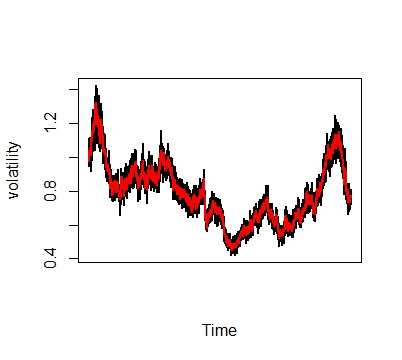
\includegraphics[width=\textwidth]{ex6_IVRV1.jpeg}
    \end{subfigure}\hfill
    \begin{subfigure}{0.32\textwidth}
        \centering
        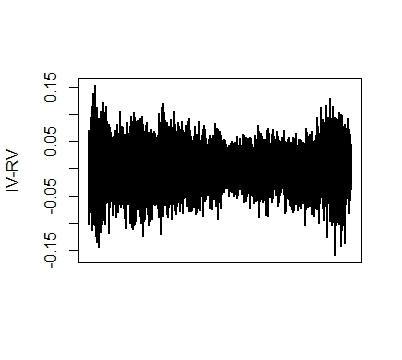
\includegraphics[width=\textwidth]{ex6_IVRV2.jpeg}
    \end{subfigure}\hfill
    \begin{subfigure}{0.32\textwidth}
        \centering
        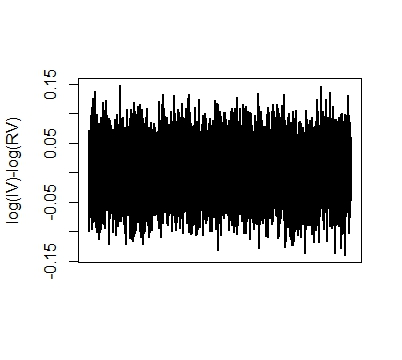
\includegraphics[width=\textwidth]{ex6_IVRV3.jpeg}
    \end{subfigure}
    \caption{Simulation from the OU-SV model. \textbf{Left:} The red line represents instantaneous volatility $\sigma_t$ whereas the black line represents realized volatility $RV_t$. \textbf{Middle:} Corresponding estimation error for the left simulated path. \textbf{Right:} Corresponding log estimation error.}
    \label{fig:example}
\end{figure}\\\\
We now compute the distributions of the estimated roughness index via normalized $p$-th statistic $\hat{H}_{L,K}$ with $L=300\times 300$ and $K=300$ for realized volatility and instantaneous volatility. We generate the distributions across 2500 independent paths drawn from the OU-SV model \eqref{eq:ousv}. The left plot of Figure \ref{fig:ex6dens} is the distribution of $\hat{H}_{L,K}$ for realized volatility whereas the right plot is the corresponding distribution for instantaneous volatility as data in the roughness estimator. In addition to this, Table \ref{tab:ex6dens} provides the summary statistics for the roughness estimator $\hat{H}_{L,K}$ for realized and instantaneous volatility respectively across the 2500 independent paths. We observe that realized volatility systematically exhibit much rougher behaviour than instantaneous volatility. The roughness estimates based on instantaneous volatility are very close to the roughness of the true model $H=0.5$. However, the roughness estimates generated from realized volatility are much smaller with a mean of $\hat{H}_{L,K}=0.1549$ across the 2500 independent simulations.
\begin{figure}[htbp]
    \centering
    
    \begin{subfigure}{0.48\textwidth}
        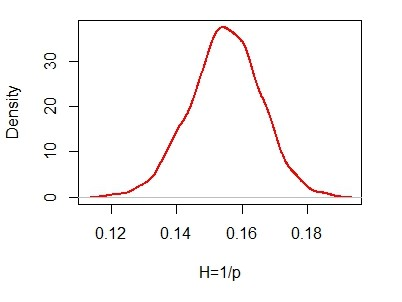
\includegraphics[width=\linewidth]{ex6_densRV.jpeg}
    \end{subfigure}
    \hfill
    \begin{subfigure}{0.48\textwidth}
        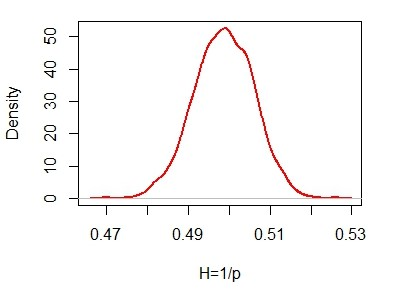
\includegraphics[width=\linewidth]{ex6_densIV.jpeg}
    \end{subfigure}
    
    \caption{Distribution of the estimated roughness index $\hat{H}_{L,K}$ via normalized $p$-th variation using $L=300\times 300$ and $K=300$ across 2500 independent simulations of the OU-SV model \eqref{eq:ousv}. \textbf{Left:} Realized volatility. \textbf{Right:} Instantaneous volatility.}
    \label{fig:ex6dens}
\end{figure}
\begin{table}[htbp]
    \centering
    \begin{tabular}{ccc}
        \toprule
         & Realized volatility & Instantaneous volatility \\
        \midrule
        Min. & 0.1192 & 0.4698 \\
        1st quartile & 0.1480 & 0.4938 \\
        Median & 0.1551 & 0.4988 \\
        Mean & 0.1549 & 0.4987 \\
        3rd quartile & 0.1621 & 0.5039 \\
        Max. & 0.1873 & 0.5257 \\
        \bottomrule
    \end{tabular}
    \caption{Summary of statistics for estimated roughness index $\hat{H}_{L,K}$ for realized and instantaneous volatility across 2500 independent simulations the OU-SV model \eqref{eq:ousv} with $L=300\times 300$ and $K=300$.}
    \label{tab:ex6dens}
\end{table}\\\\
Note that our results deviates slightly from the results in \cite{cont} for a similar model. This might be caused by \cite{cont} using the mean of $\sigma_t$ across the 300 consecutive data points as their instantaneous volatility which seems to create a slightly smoother volatility process. Furthermore, \cite{cont} might be using a different $T$ than us which in the OU-SV model will significantly impact the size of the estimation error and thus the estimated roughness index for realized volatility when all other parameters are kept constant. The conclusions are however the same. Realized volatility does systematically exhibit much rougher behaviour than instantaneous volatility and than the true roughness of the model. This rougher behaviour is solely caused by the estimation error, and it indicates that roughness estimated based on realized volatility can be unreliable.

\subsection{A fractional Ornstein-Uhlenbeck model}
In the two previous models, instantaneous volatility follows a diffusive behaviour similar to a Brownian motion with $H=0.5$. We now consider a more general case of a stochastic volatility model where the volatility process has a general roughness index $H\in(0,1)$ generated from a fractional Brownian motion. We investigate the model for different roughness indexes and explore how this affect the estimation error and estimated roughness index. Consider the following process where the volatility is described by a fractional Ornstein-Uhlenbeck model:
\begin{align}
dS_t = S_t \sigma_t dB_t, \quad \sigma_t = \sigma_0 e^{Y_t}, \quad dY_t = -\gamma Y_t \, dt + \theta \, dB^H_t, \label{eq:fou}
\end{align}
where $S_t$ is the price process, $B_t$ is a Brownian motion, and $B_t^H$ is a fractional Brownian motions with Hurst exponent $H$. For the simulation we use the parameters $\sigma_0 =\gamma=\theta=1$ and $Y_0=0$, and we set $T=5$ and $S_0=1$.\\\\
We now repeat the procedure described in section 4.1 to compute the estimated roughness index $\hat{H}_{L,K}$ with $L=300\times 300$ and $K=300$ for realized and instantaneous volatility. Furthermore, we compute the smoothness parameter from section 3.5 for both the realized and instantaneous volatility. We compute these roughness estimates across different values of the true Hurst exponent $H$. In Table \ref{tab:ex7table} we have computed roughness estimates from the fractional Ornstein-Uhlenbeck model \eqref{eq:fou} with Hurst exponent $H=\{0.1,0.2,0.3,0.4,0.5,0.6,0.7,0.8\}$. We have used the same seed in the simulation for all values of $H$ such that the underlying stochastic element of the price processes are the same. Thus, the difference between the price processes solely lies in the Hurst exponent $H$.
\begin{table}[htbp]
    \centering
    \begin{tabular}{cccccc}
        \toprule
        H & Instantaneous vol & Realized vol & IV (log reg) & RV (log reg)\\
        \midrule
        0.1 & 0.126 & 0.199 & 0.102 & 0.197\\
        0.2 & 0.220 & 0.256 & 0.204 & 0.250\\
        0.3 & 0.313 & 0.261 & 0.305 & 0.257\\
        0.4 & 0.408 & 0.218 & 0.407 & 0.188\\
        0.5 & 0.504 & 0.159 & 0.508 & 0.095\\
        0.6 & 0.598 & 0.102 & 0.607 & 0.036\\
        0.7 & 0.691 & 0.070 & 0.703 & 0.012\\
        0.8 & 0.778 & 0.052 & 0.794 & 0.004\\
        \bottomrule
    \end{tabular}
    \caption{Estimated roughness via $p$-th variation $\hat{H}_{L,K}$ and via log regression for instantaneous and realized volatility for simulated data from a fractional Ornstein-Uhlenbeck model \eqref{eq:fou} with Hurst exponent $H=\{0.1,0.2,0.3,0.4,0.5,0.6,0.7,0.8\}$.}
    \label{tab:ex7table}
\end{table}\\\\
The corresponding paths for price process, realized volatility and instantaneous volatility from model \ref{eq:fou} with Hurst exponent $H=\{0.1,0.2,0.3,0.4,0.5,0.6,0.7,0.8\}$ are presented in Figure \ref{fig:ex7paths}. Visually we observe that the price processes do not differ much as the Hurst exponent changes. However, the paths of realized and instantaneous volatility are very different for different Hurst exponents. For small Hurst exponents instantaneous volatility does visually appear more rough than realized volatility. However, instantaneous volatility becomes smoother and smoother as $H$ increases. That is expected since increasing the Hurst exponent $H$ exactly means that the volatility process becomes smoother. However, realized volatility is not gradually getting smoother as $H$ increases. Instead we observe that for large Hurst exponents, realized volatility appears very rough. This is supported by the estimated roughness indices in Table \ref{tab:ex7table}. The estimated roughness based on instantaneous volatility is increasing as $H$ increases both for the roughness estimator via $p$-th variation and the estimator via logarithmic regression. The estimated roughness based on realized volatility is increasing at first as $H$ increases, but for large Hurst exponents the estimated roughness decreases and the estimated roughness of the volatility process is estimated to be very rough when the true Hurst exponent is $H=0.8$. 
\begin{figure}[htbp]
    \centering
    
    \begin{subfigure}{0.32\textwidth}
        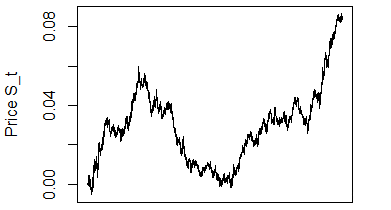
\includegraphics[width=\linewidth]{H01_S.png}
    \end{subfigure}
    \hfill
    \begin{subfigure}{0.32\textwidth}
        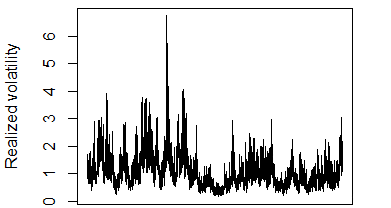
\includegraphics[width=\linewidth]{H01_RV.png}
    \end{subfigure}
    \hfill
    \begin{subfigure}{0.32\textwidth}
        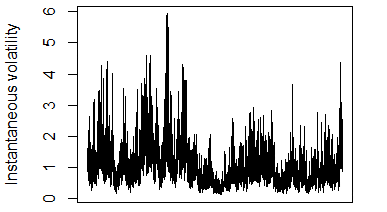
\includegraphics[width=\linewidth]{H01_IV.png}
    \end{subfigure}
    \vskip 0em
    \begin{subfigure}{0.32\textwidth}
        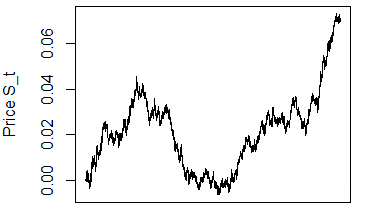
\includegraphics[width=\linewidth]{H02_S.png}
    \end{subfigure}
    \hfill
    \begin{subfigure}{0.32\textwidth}
        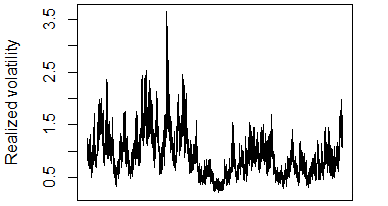
\includegraphics[width=\linewidth]{H02_RV.png}
    \end{subfigure}
    \hfill
    \begin{subfigure}{0.32\textwidth}
        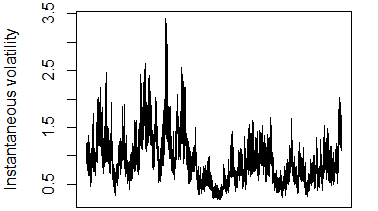
\includegraphics[width=\linewidth]{H02_IV.png}
    \end{subfigure}
        \vskip 0em
    \begin{subfigure}{0.32\textwidth}
        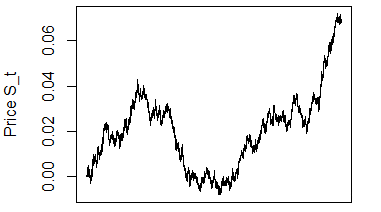
\includegraphics[width=\linewidth]{H03_S.png}
    \end{subfigure}
    \hfill
    \begin{subfigure}{0.32\textwidth}
        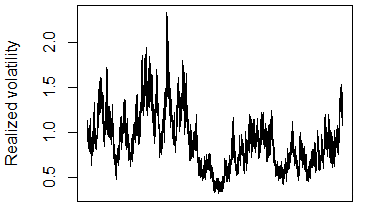
\includegraphics[width=\linewidth]{H03_RV.png}
    \end{subfigure}
    \hfill
    \begin{subfigure}{0.32\textwidth}
        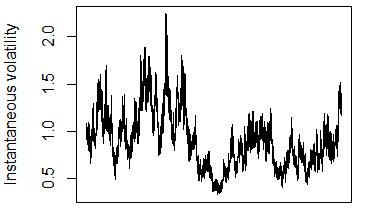
\includegraphics[width=\linewidth]{H03_IV.png}
    \end{subfigure}
        \vskip 0em
    \begin{subfigure}{0.32\textwidth}
        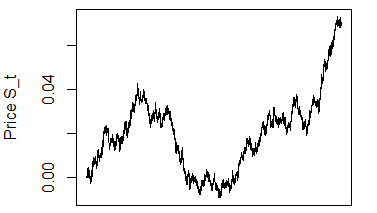
\includegraphics[width=\linewidth]{H04_S.png}
    \end{subfigure}
    \hfill
    \begin{subfigure}{0.32\textwidth}
        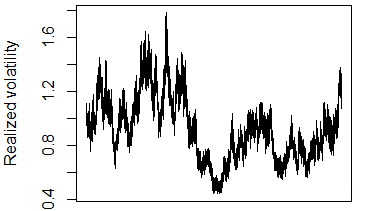
\includegraphics[width=\linewidth]{H04_RV.png}
    \end{subfigure}
    \hfill
    \begin{subfigure}{0.32\textwidth}
        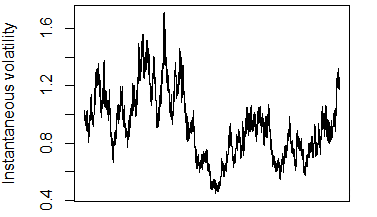
\includegraphics[width=\linewidth]{H04_IV.png}
    \end{subfigure}
        \vskip 0em
    \begin{subfigure}{0.32\textwidth}
        \includegraphics[width=\linewidth]{H05_S.png}
    \end{subfigure}
    \hfill
    \begin{subfigure}{0.32\textwidth}
        \includegraphics[width=\linewidth]{H05_RV.png}
    \end{subfigure}
    \hfill
    \begin{subfigure}{0.32\textwidth}
        \includegraphics[width=\linewidth]{H05_IV.png}
    \end{subfigure}
        \vskip 0em
    \begin{subfigure}{0.32\textwidth}
        \includegraphics[width=\linewidth]{H06_S.png}
    \end{subfigure}
    \hfill
    \begin{subfigure}{0.32\textwidth}
        \includegraphics[width=\linewidth]{H06_RV.png}
    \end{subfigure}
    \hfill
    \begin{subfigure}{0.32\textwidth}
        \includegraphics[width=\linewidth]{H06_IV.png}
    \end{subfigure}
        \vskip 0em
    \begin{subfigure}{0.32\textwidth}
        \includegraphics[width=\linewidth]{H07_S.png}
    \end{subfigure}
    \hfill
    \begin{subfigure}{0.32\textwidth}
        \includegraphics[width=\linewidth]{H07_RV.png}
    \end{subfigure}
    \hfill
    \begin{subfigure}{0.32\textwidth}
        \includegraphics[width=\linewidth]{H07_IV.png}
    \end{subfigure}
        \vskip 0em
    \begin{subfigure}{0.32\textwidth}
        \includegraphics[width=\linewidth]{H08_S.png}
    \end{subfigure}
    \hfill
    \begin{subfigure}{0.32\textwidth}
        \includegraphics[width=\linewidth]{H08_RV.png}
    \end{subfigure}
    \hfill
    \begin{subfigure}{0.32\textwidth}
        \includegraphics[width=\linewidth]{H08_IV.png}
    \end{subfigure}
    
    \caption{ \textbf{Left:} Simulated price path $S_t-S_0$ of fractional OU model \ref{eq:fou} with Hurst exponent $H=\{0.1,0.2,0.3,0.4,0.5,0.6,0.7,0.8\}$ respectively. \textbf{Center:} Realized volatility. \textbf{Right:} Instantaneous volatility.}
    \label{fig:ex7paths}
\end{figure}\\\\
In Figure \ref{fig:ex7single} we have plotted the values from Table \ref{tab:ex7table} in a graph. The blue lines represents roughness estimates for instantaneous volatility while the red lines represents roughness estimates for the corresponding realized volatility. The solid lines are the estimated roughness index via $p$-th variation $\hat{H}_{L,K}$ with $L=300\times 300$ and $K=300$ while the dashed lines represent roughness estimates using the smoothness parameter computed by logarithmic regression. The $x$-axis represent the true value of $H$ of the simulated fractional OU model. We observe that roughness estimates based on instantaneous volatility give accurate estimates of the true Hurst index $H$. However, the estimated roughness for realized volatility is quite inaccurate and always stay below $0.3$. In particular, when the instantaneous volatility process is generated from a smooth process (i.e. $H>\frac{1}{2}$) the roughness estimate of realized volatility turns out to be a very poor estimate.\\ 
It seems that our two roughness estimates coincides and generate similar estimates. Only when the true model is smooth (i.e. $H>0.5$) the roughness estimate by logarithmic regression for realized volatility seems to systematically be rougher that the corresponding roughness estimate via $p$-th variation. However, both estimates are very poor in this case. 
\begin{figure}[htbp]
    \centering
    
    \begin{subfigure}{0.78\textwidth}
        \includegraphics[width=\linewidth]{ex7_single_plot.png}
    \end{subfigure}
    
    \caption{Estimated roughness indexes for realized and instantaneous volatility from a fractional OU model (\ref{eq:fou}) plotted for price paths generated by different values of $H$. The solid lines are roughness indexes via $p$-th variation $\hat{H}_{L,K}$ with $L = 300\times 300$ and $K= 300$ while the dashed lines represents estimated roughness by logarithmic regression.}
    \label{fig:ex7single}
\end{figure}\\\\
In Figure \ref{fig:ex7plot100} we have repeated the above analyses for 100 independent simulated prices processes generated by the fractional Ornstein-Uhlenbeck model \ref{eq:fou} but only for the estimated roughness index via $p$-th variation $\hat{H}_{L,K}$ with $L = 100\times 100$ and $K= 100$. The figure shows the estimators $\hat{H}_{L,K}(RV)$ and $\hat{H}_{L,K}(\sigma)$ plotted against Hurst exponents $H=\{0.1,0.2,0.3,0.4,0.5,0.6,0.7,0.8\}$ for every independent path. The bold black lines represent the mean across 100 independent simulations whereas the dotted lines represent the corresponding 75\% confidence interval. If equation \ref{eq:wpth} have no solution for $H\in (0,1)$ we set $\hat{H}_{L,K}=0$.
\begin{figure}[htbp]
    \centering
    
    \begin{subfigure}{0.78\textwidth}
        \includegraphics[width=\linewidth]{ex7_plot100.png}
    \end{subfigure}
    
    \caption{Estimated roughness index via $p$-th variation for realized and instantaneous volatility plotted against different values of $H$ for 100 independent price paths from a fractional OU model (\ref{eq:fou}). The solid black lines represent the mean across the 100 paths and the dashed black lines represent the corresponding 75\% confidence interval.}
    \label{fig:ex7plot100}
\end{figure}\\\\
From Figure \ref{fig:ex7plot100} we observe that for all 100 independent simulations the roughness estimators exhibit a similar behaviour. Our conclusions about the poorness of roughness estimates for realized volatility still hold and was not just a matter of the single price path we studied before. In particular, for the fractional Ornstein-Uhlenbeck model \ref{eq:fou} realized volatility always exhibit rough behaviour (i.e. $H<\frac{1}{2}$) no matter what the true roughness of the volatility process is. The estimated roughness based on instantaneous volatility is quite accurate and as this is a simulation study we have no measurement errors so the inaccuracy of the estimators for realized volatility solely comes from the estimation error. \\\\
In practice, instantaneous volatility cannot be observed, and roughness estimates are based on realized volatility. However, the above examples illustrate that one cannot necessarily draw the conclusion that (spot) volatility is rough just because realized volatility exhibit rough behaviour with $\hat{H}_{L,K}(RV)<\frac{1}{2}$ even if the estimated roughness is well below $\frac{1}{2}$.

\subsection{RFSV model}
We will now consider the stochastic volatility model suggested by \cite{gatheral}. The model is defined in the following way:
\begin{align}
dS_t = S_t \sigma_t \sqrt{dt}U_n, \quad \sigma_t = e^{Y_t}, \quad dY_t = -\alpha (Y_t-m) \, dt + \nu \, dB^H_t, \label{eq:rfsv}
\end{align}
for some $\nu>0$, $\alpha>0$, $m\in\mathbb{R}$ and $H<\frac{1}{2}$ where $B^H_t$ is a fractional Brownian motion and $U_n$ are iid standard Gaussian variables. \cite{gatheral} further argues that choosing $\alpha \ll \frac{1}{T}$ is desirable since the log-volatility then locally behaves like a fBm while it is still technically stationary. In addition to this, \cite{gatheral} argues that observed skew term structure in financial data can easier be replicated by choosing $\alpha \ll \frac{1}{T}$.\\\\
The specified RFSV model is similar to model (\ref{eq:fou}) from section 4.3 and both models use a fractional Ornstein-Uhlenbeck process to model log-volatility. In this section we use a different approach to compute realized and instantaneous volatility. We follow much of the simulation approach from \cite{gatheral}. We set $T=3601$ and simulate 5000 point per day. For every day we compute the realized volatility of the first 1000 points of the day, and we then rescale this volatility to be a daily volatility estimate. The corresponding instantaneous volatility is computed as the mean of the first 1000 points per day. Following this approach to compute volatility data, we perform many of the same analyses as in section 4.3. When simulating from the model we use the parameters $\nu = 0.2$, $\alpha = 10^{-4}$, $m = -7$ and we set $Y_0=m$ and $S_0 = 1$.\\\\
In Table (++) we have computed roughness estimates from the RSFV model (\ref{eq:rfsv}) with Hurst exponent $H= \{0.1,0.2,0.3,0.4,0.5\}$.
\begin{table}[htbp]
    \centering
    \begin{tabular}{cccccc}
        \toprule
        H & Instantaneous vol & Realized vol & IV (log reg) & RV (log reg)\\
        \midrule
        0.1 & 0.175 & 0.168 & 0.146 & 0.143\\
        0.2 & 0.241 & 0.236 & 0.217 & 0.214\\
        0.3 & 0.314 & 0.310 & 0.297 & 0.295\\
        0.4 & 0.394 & 0.390 & 0.386 & 0.384\\
        0.5 & 0.475 & 0.472 & 0.478 & 0.476\\
        \bottomrule
    \end{tabular}
    \caption{Estimated roughness via $p$-th variation $\hat{H}_{L,K}$ with $L=60\times60$ and $K=60$ and via log regression for instantaneous and realized volatility for simulated data from the RSFV model \eqref{eq:rfsv} with Hurst exponent $H=\{0.1,0.2,0.3,0.4,0.5\}$.}
    \label{tab:ex7table}
\end{table}
\begin{figure}[htbp]
    \centering
    
    \begin{subfigure}{0.78\textwidth}
        \includegraphics[width=\linewidth]{rsfv_single.jpeg}
    \end{subfigure}
    
    \caption{Estimated roughness indexes for realized and instantaneous volatility from a RSFV model (\ref{eq:fou}) plotted for price paths generated by different values of $H$. The solid lines are roughness indexes via $p$-th variation $\hat{H}_{L,K}$ with $L = 3600$ and $K= 60$ while the dashed lines represents estimated roughness by logarithmic regression.}
    \label{fig:rsfv_single}
\end{figure}\\\\

\newpage
\section{Appendix}
\subsection{A Spectral Method FFT}
Consider 
\[
a_k := \begin{cases}
0 & k = 0; \\
\frac{1}{2} \left( U^{(0)}_{k-1} + i U^{(1)}_{k-1} \right) \sqrt{\frac{f(t_k)}{\ell}} & k = 1, \dots, \ell - 1; \\
U^{(0)}_{k-1} \sqrt{\frac{f(t_k)}{\ell}} & k = \ell; \\
\frac{1}{2} \left( U^{(0)}_{2\ell - k - 1} - i U^{(1)}_{2\ell - k - 1} \right) \sqrt{\frac{f(t_{2\ell - k})}{\ell}} & k = \ell + 1, \dots, 2\ell - 1.
\end{cases}
\]
We want to take the Fourier transform of this sequence. The Fourier transform of $(a_k)_{k=0}^{2\ell-1}$ is $\lambda_n = \sum_{k=0}^{2\ell-1} a_k \exp(2\pi i \frac{nk}{2\ell})$. By Euler's formula we obtain
\begin{align*}
\lambda_n = \sum_{k=0}^{2\ell-1} a_k \left( \cos\left(\pi\frac{nk}{\ell}\right) + i\sin\left(\pi \frac{nk}{\ell}\right)\right).
\end{align*}
We will now insert $a_k$ and split the sum into the four different cases of $a_k$. Hence, we obtain
\begin{align*}
&\lambda_n = 0 + \sum_{k=1}^{l-1} \frac{1}{2} \left( U^{(0)}_{k-1} + i U^{(1)}_{k-1} \right) \sqrt{\frac{f(t_k)}{\ell}} \left( \cos\left(\pi\frac{nk}{\ell}\right) + i\sin\left(\pi \frac{nk}{\ell}\right)\right)\\
&+ U^{(0)}_{\ell-1} \sqrt{\frac{f(t_\ell)}{\ell}}\left( \cos\left(\pi\frac{n\ell}{\ell}\right) + i\sin\left(\pi \frac{n\ell}{\ell}\right)\right)\\
&+ \sum_{k=l+1}^{2l-1} \frac{1}{2} \left( U^{(0)}_{2\ell - k - 1} - i U^{(1)}_{2\ell - k - 1} \right) \sqrt{\frac{f(t_{2\ell - k})}{\ell}}\left( \cos\left(\pi\frac{nk}{\ell}\right) + i\sin\left(\pi \frac{nk}{\ell}\right)\right).
\end{align*}
By definition $t_k=\frac{\pi k}{\ell}$. Thus, what is inside the cosine and sine functions is simply $nt_k$. Note that for $k=\ell$ we have $t_k=\pi$. Thus, $\sin(nt_\ell)=0$ since $n$ is an integer. By inserting this and changing the indexes of the two sums, we obtain
\begin{align*}
&\lambda_n = U^{(0)}_{\ell-1} \sqrt{\frac{f(t_\ell)}{\ell}}\cos(nt_\ell)\\
& + \sum_{k=0}^{l-2} \frac{1}{2} \left( U^{(0)}_{k}+ i U^{(1)}_{k} \right) \sqrt{\frac{f(t_{k+1})}{\ell}} \left( \cos\left(n t_{k+1}\right) + i\sin\left(n t_{k+1}\right)\right)\\
&+ \sum_{k=0}^{l-2}\frac{1}{2} \left( U^{(0)}_{\ell-k-2}- i U^{(1)}_{\ell-k-2} \right) \sqrt{\frac{f(t_{\ell-k-1})}{\ell}} \left( \cos\left(n t_{\ell+k+1}\right) + i\sin\left(n t_{\ell+k+1}\right)\right).
\end{align*}
Now note that $\sin\left(n t_{\ell+k+1}\right) = -\sin(nt_{\ell-(k+1)})$ since $t_\ell = \pi$. Similarly, $\cos\left(n t_{\ell+k+1}\right) = \cos(nt_{\ell-(k+1)})$. By inserting that in the last sum in the above expression, the sum becomes
\begin{align*}
&\sum_{k=0}^{l-2}\frac{1}{2} \left( U^{(0)}_{\ell-k-2}- i U^{(1)}_{\ell-k-2} \right) \sqrt{\frac{f(t_{\ell-k-1})}{\ell}} \left( \cos\left(n t_{\ell-k-1}\right) - i\sin\left(n t_{\ell-k-1}\right)\right)\\
& =\sum_{k=0}^{l-2}\frac{1}{2} \left( U^{(0)}_{k}- i U^{(1)}_{k} \right) \sqrt{\frac{f(t_{k+1})}{\ell}} \left( \cos\left(n t_{k+1}\right) - i\sin\left(n t_{k+1}\right)\right)
\end{align*}
where we have reversed the sum order. Now we can combine the two sums into one. Several terms cancel out such that we obtain
\begin{align*}
&\lambda_n = U^{(0)}_{\ell-1} \sqrt{\frac{f(t_\ell)}{\ell}}\cos(nt_\ell)+ \sqrt{\frac{f(t_{k+1})}{\ell}} \sum_{k=0}^{l-2} \left(U^{(0)}_k\cos\left(n t_{k+1}\right)-U^{(1)}_{k}\sin\left(n t_{k+1}\right)\right)\\
& = \sum_{k=0}^{l-1}\sqrt{\frac{f(t_{k+1})}{\ell}}\left(U^{(0)}_k\cos\left(n t_{k+1}\right)-U^{(1)}_{k}\sin\left(n t_{k+1}\right)\right)
\end{align*}
which equals the definition of $\hat{X}_n^{(\ell)}$ from (11) as desired.

\newpage
\addcontentsline{toc}{section}{References}
\bibliographystyle{plainnat}
\setcitestyle{round}
\bibliography{masterRef}
\end{document}